%% Type de document et encodage de la police
\documentclass[a4paper]{article}
\usepackage[utf8x]{inputenc}

%% Initialise la taille des pages et des marges
\usepackage[a4paper,top=3cm,bottom=3cm,left=2cm,right=2cm,marginparwidth=1.75cm]{geometry}

%% Packs utiles
\usepackage{amsmath}
\usepackage{graphicx}
\usepackage[colorinlistoftodos]{todonotes}
\usepackage[colorlinks=true, allcolors=black]{hyperref}
\usepackage{fourier-orns}
\usepackage{titlesec}
\usepackage{fancyhdr}
\usepackage{fancyvrb}
\usepackage{array}
\usepackage{cancel}
\usepackage{upgreek}
\usepackage{arydshln}
\usepackage{mathtools}% superior to amsmath

%% Packs utiles pour la manipulation d'image
\usepackage{wallpaper}
\usepackage{amsfonts}
\usepackage{amssymb}
\usepackage{eso-pic}
\usepackage{multicol}
\usepackage{wrapfig}

%% \setlength
\setlength{\parindent}{0.5cm}

%% \thefootnote
\renewcommand{\thefootnote}{\*}
\pagestyle{fancy} 
\setcounter{tocdepth}{5}
\renewcommand{\thefootnote}{\arabic{footnote}}

%% \headrulewidth
\renewcommand{\headrulewidth}{1pt}
\fancyhead[C]{} 
\fancyhead[L]{}
\fancyhead[R]{\footnotesize{\leftmark}}

%% \footrulewidth
\renewcommand{\footrulewidth}{1pt}
\fancyfoot[C]{} 
\fancyhead[L]{}
\fancyfoot[R]{\thepage}

%% definecolor
\definecolor{Zgris}{rgb}{0.87,0.85,0.85}

%% Pour mettre des lignes à gauche et à droite d'un exemple
\usepackage{mdframed}
\newmdenv[
  topline=false,
  bottomline=false,
  skipabove=\topsep,
  skipbelow=\topsep
]{siderules}

%% Redéfinition de la colonne d'un tableau pour que ses éléments soient centrés sur l'axe vertical
%% Implique l'utilisation de \tabularnewline à la place de \\ pour terminer une ligne du tableau
\newcolumntype{M}[1]{>{\raggedright}m{#1}}

%% Pack Tikz pour les diagrammes
\usepackage{tikz}
\usetikzlibrary{shapes.geometric, arrows, shapes, shapes.multipart, decorations.pathmorphing, backgrounds, positioning, fit, petri}
\usetikzlibrary{calc,patterns,decorations.pathreplacing,decorations.markings,3d,backgrounds,tikzmark}

%% Noeud start -> diagrammes
\tikzstyle{start} = [rectangle, rounded corners, minimum width = 3cm, minimum height = 1cm, text centered, draw = black, fill = red!30]

%% Pack circuitikz pour les circuits électriques
\usepackage{circuitikz}

%% Utilisation de \mathpzc{}
\DeclareMathAlphabet{\mathpzc}{OT1}{pzc}{m}{it}

%% Pour faire un encadré au coins arrondis
\usepackage{fancybox}
\cornersize{0.25}

%% Pour mettre deux cercles au-dessus d'une lettre \ringring{}
\newcommand\ringring[1]{%
  {% make an Ord atom
   \mathop{\kern0pt #1}\limits^{% set a box over the variable
     \vbox to-1.85ex{
       \kern-2ex % lower the ring accents
       \hbox to 0pt{\hss\normalfont\kern.1em \r{}\kern-.45em \r{}\hss}%
       \vss % fill
     }% end of \vbox
   }% end of the superscript
  }% end of \mathop
}

%% Pour ignorer le itemize
\newcommand\NoIndent[1]{%
  \par\vbox{\parbox[t]{\linewidth}{#1}}%
}

%% Dessiner des cercles irréguliers
\newcommand\irregularcircle[2]{% radius, irregularity
  \pgfextra {\pgfmathsetmacro\len{(#1)+rand*(#2)}}
  +(0:\len pt)
  \foreach \a in {10,20,...,350}{
    \pgfextra {\pgfmathsetmacro\len{(#1)+rand*(#2)}}
    -- +(\a:\len pt)
  } -- cycle
}










%% Titre, auteur, date
\title{Mécanique rationnelle}
\author{Grégoire Roumache}
\date{Janvier 2018}












%% Début document
\begin{document}



%% Fait apparaître le titre
\maketitle
















\section{Théorie : Notions fondamentales - Point matériel}











\begin{itemize}









%% Point matériel et vecteur position
\item Un point matériel P est un corps ponctuel sans surface ni volume mais possédant une masse constante. Il est relié à l'origine du repère O par le vecteur \textbf{OP} aussi noté \textbf{s} qui est le vecteur position du point P. La relation $ \textbf{s} = \textbf{s}(t) $ est appelée "Loi du mouvement".





%% Vitesse et accélération
\item On définit la vitesse d'un point P par 
\[ \textbf{v}(t) = \dot{\textbf{s}}(t) = \frac{d \textbf{s}}{d t} = \lim_{\Delta t \to 0} \frac{\textbf{s}(t + \Delta t) - \textbf{s}(t)}{\Delta t} \]
et son accélération par 
\[ \textbf{a}(t) = \ddot{\textbf{s}}(t) = \frac{d \textbf{v}}{d t} = \lim_{\Delta t \to 0} \frac{\textbf{v}(t + \Delta t) - \textbf{v}(t)}{\Delta t} \]





%% Trièdre local de Frenet
\item L'abscisse curviligne $ \lambda $ est mesurée le long de la courbe à partir d'un point quelconque pris comme origine, on peut noter $ \textbf{s} = \textbf{s}(\lambda) $. \\
Le trièdre local de Frenet est formé par : 
\begin{enumerate}
\item Le vecteur unitaire selon la tangente à la courbe : $\displaystyle \boldsymbol{\tau} = \frac{d \textbf{s}}{d \lambda} $.
\item Le vecteur unitaire selon la normale principale : $\displaystyle \boldsymbol{\nu} = \rho \frac{d \boldsymbol{\tau}}{d \lambda} $.
\item Le vecteur unitaire selon la binormale : $\displaystyle \boldsymbol{\beta} = \boldsymbol{\tau} \wedge \boldsymbol{\nu} $
\end{enumerate}





%% Formule de Poisson
\item Soient les référentiels $ (O, \textbf{E}_1, \textbf{E}_2, \textbf{E}_3) $ et $ (O', \textbf{e}_1, \textbf{e}_2, \textbf{e}_3) $. Adoptons le repère de centre O comme repère de base. Le mouvement des vecteurs (unitaires) liés en O' par rapport au vecteurs de O ne peut être qu'une rotation. \\
La dérivée du vecteur $ \textbf{e}_i $ lui est perpendiculaire et peut donc s'écrire : $\displaystyle \bigg( \frac{d \textbf{e}_i}{d t} \bigg)_O = \textbf{w} \wedge \textbf{e}_i $. \\
Le vecteur \textbf{w} est unique et peut être utilisé pour exprimer les dérivées temporelles de tous les vecteurs unitaires de la base. \textbf{w} est appelé "vecteur de Poisson" ou "vecteur vitesse de rotation". La formule $\displaystyle \bigg( \frac{d \textbf{e}_i}{d t} \bigg)_O = \textbf{w} \wedge \textbf{e}_i $ est appelée "formule de Poisson". On généralise la formule de Poisson à l'accélération : $\displaystyle \bigg( \frac{d \textbf{a}}{d t} \bigg)_O = \bigg( \frac{d \textbf{a}}{d t} \bigg)_{O'} + \textbf{w} \wedge \textbf{a} $.





%% Décomposition de la vitesse
\item Soit $ \textbf{b} = \textbf{OO'} $, $ \textbf{s} = \textbf{OP} $ et $ \textbf{r} = \textbf{O'P} $. On a évidemment la relation $\displaystyle \frac{d \textbf{s}}{d t} = \frac{d \textbf{b}}{d t} + \frac{d \textbf{r}}{d t} $, en y appliquant la formule de Poisson, on obtient : 
\[ \dot{\textbf{s}} = \underbrace{\dot{\textbf{b}} + \textbf{w} \wedge \textbf{r}}_{\textbf{v}_e} + \underbrace{\frac{\delta \textbf{r}}{\delta t}}_{\textbf{v}_r} \]
où $\displaystyle \frac{\delta}{\delta t} $ désigne la dérivée relative évaluée dans la base mobile, $ \textbf{v}_r $ est la vitesse relative et $ \textbf{v}_e $ est la vitesse d'entraînement. \\





%% Décomposition de l'accélération
\item Une décomposition semblable peut être effectuée pour l'accélération : 
\[ \frac{d^2 \textbf{s}}{d t^2} = \underbrace{ \frac{d^2 \textbf{b}}{d t^2} + \dot{\textbf{w}} \wedge \textbf{r} + \textbf{w} \wedge (\textbf{w} \wedge \textbf{r}) }_{\textbf{a}_e} + \underbrace{ 2 \; \textbf{w} \wedge \frac{\delta \textbf{r}}{\delta t} }_{\textbf{a}_c} + \underbrace{ \frac{\delta^2 \textbf{r}}{\delta t^2} }_{\textbf{a}_r} \]
où $ \textbf{a}_e $ est l'accélération d'entraînement, $ \textbf{a}_c $ est l'accélération de Coriolis et $ \textbf{a}_r $ est l'accélération relative.





%% Grandeurs cinématiques associées
\item En plus de la masse m (ou $ d m $), la position $ \textbf{s} $ et la vitesse $ \dot{\textbf{s}} $, il est d'usage d'introduire d'autres grandeurs caractéristiques : 
\begin{enumerate}
\item Le moment statique : $\displaystyle \textbf{Q}_O = m \; \textbf{s} $.
\item La quantité de mouvement : $\displaystyle \textbf{N}_O = m \; \dot{\textbf{s}} $.
\item Le moment cinétique : $\displaystyle \textbf{H}_O = m \; \textbf{s} \wedge \dot{\textbf{s}} $.
\item L'énergie cinétique : $\displaystyle T_O = \frac{1}{2} m \; \| \dot{\textbf{s}} \|^2 $.
\end{enumerate}
Les symboles désignant ces grandeurs sont munis d'un indice rappelant le système d'axes auquel elles se rapportent.





%% Grandeurs dynamiques associées
\item On définit des grandeurs dynamiques qui ont un rôle important en mécanique : 
\begin{enumerate}
\item Le moment dynamique : $\displaystyle \textbf{M}_O = \textbf{s} \wedge \textbf{F} $.
\item La puissance : $\displaystyle \mathpzc{P}_O = \dot{\textbf{s}} \cdot \textbf{F} $.
\item La résultante : $\displaystyle \textbf{G} = \sum_i \textbf{F}_i + \int \hat{\textbf{F}} \; d m $.
\item Le moment résultant : $\displaystyle \textbf{M}_O = \sum_i \textbf{s}_i \wedge \textbf{F}_i + \int \textbf{s} \wedge \hat{\textbf{F}} \; d m $.
\end{enumerate}





%% Forces données
\item L'expression mathématique de beaucoup de forces responsables du mouvement est connue dès l'abord du problème : 
\begin{enumerate}
\item Champ de force : Le vecteur force $ \textbf{F}(\textbf{s}) $ est donné en chaque point $ \dot{\textbf{S}} $ d'une région déterminée de l'espace. Un exemple important est le champ gravitationnel. La force est dans ce cas : $\displaystyle \hat{\textbf{F}}(\textbf{s}) = - \frac{\mu}{s^3} \textbf{s} $ \qquad où \qquad $ \mu > 0 $, \qquad $ s = \| \textbf{s} \| $.
\item Force de rappel d'un ressort : $\displaystyle \textbf{F} = - k \; (l - l_0) \; \textbf{e} $. \\
De même pour un ressort de torsion d'axe \textbf{e} : $\displaystyle \textbf{C} = - k \; (\theta - \theta_0) \; \textbf{e} $.
\item Tension dans une corde élastique : Comme dans le cas du ressort, on considère que la tension dans une corde élastique est proportionnelle à l'extension de celle-ci. A la différence que la tension ne s'exerce que lorsque la corde est tendue et étirée.
\item Force de frottement fluide : Dans le cas le plus simple, on a : $\displaystyle \textbf{F} = - c \; \dot{\textbf{s}} $ \; (loi de Stokes).
\item Force de Lorentz : $\displaystyle \textbf{F} = q \; (\textbf{E} + \dot{\textbf{s}} \wedge \textbf{B}) $.
\end{enumerate}





%% Liaisons et forces de liaison
\item Les relations restrictives imposées à la position ou au mouvement d'un système sont appelées relations de liaisons (exemple : un point matériel qui ne peut se déplacer que sur une courbe ou une surface). Ces contraintes sont imposées par le biais de forces qui sont dés lors appelées forces de liaisons. Notamment, les forces de réaction s'exercent à l'endroit de contact entre deux corps.





%% Loi de frottement
\item Selon la loi de frottement, la force de frottement \textbf{T} agissant sur un point est donnée par : $\displaystyle \textbf{T} = - \mu \; N \; \frac{\textbf{v}}{\| \textbf{v} \|} $.





%% Liaison pivot
\item Dans le cas d'une liaison pivot (exemple : tambour qui tourne dans la cuve d'un lave-linge), sous l'action du frottement, on aura $\displaystyle \textbf{C}_F = - \mu^{\Omega} \; \text{sign}(\dot{\theta}) \; \| \textbf{R} \| \; \textbf{e} $ qui freinera le mouvement relatif du solide par rapport à l'autre.





%% Liaison glissière
\item Dans le cas d'une liaison glissière (exemple : la cabine qui bouge dans la cage d'ascenseur), sous l'action du frottement, on aura la réaction $\displaystyle \textbf{T} = - \mu \; \text{sign}(\dot{x}) \; \| \textbf{R} \| \; \textbf{e} $.





%% Forces intérieures/extérieures & Action/Réaction
\item On note les forces intérieures émanant d'éléments appartenant au système par un \textbf{f} et les forces extérieures par un \textbf{F}.
Le principe d'action/réaction s'écrit : $\displaystyle \textbf{f}_{ij} = - \textbf{f}_{ji} $.





%% Puissance
\item La puissance développée par une force quelconque \textbf{F} s'appliquant en un point de vitesse $ \dot{\textbf{s}} $ dans un repère de centre O est donnée par $\displaystyle \mathpzc{P}_O = \textbf{F} \cdot \dot{\textbf{s}} $.





%% Forces conservatives
\item Une force \textbf{F} est conservative si elle est de la forme : $\displaystyle \textbf{F} = - \nabla V $ \qquad où V est une fonction de \textbf{s}. \\
La puissance d'une force conservative est donnée par : $\displaystyle \mathpzc{P}_O = \textbf{F} \cdot \dot{\textbf{s}} = - \dot{\textbf{s}} \cdot \textbf{F} = - \frac{d V}{d t} $. Et son travail par : $\displaystyle \mathpzc{T} = \int_A^B \textbf{F} \cdot d \textbf{s} = V(\textbf{s}_B) - V(\textbf{s}_A) $.





%% Force qui ne travaille pas
\item Si la puissance développée par une force \textbf{F} est nulle, on dit que la force ne travaille pas.





%% Force dissipative
\item Une force est dite dissipative si elle développe une puissance définie négative et dissipe (en chaleur) une partie de l'énergie du système. C'est le cas des forces de résistances dans un fluide.





%% Résultantes cinématiques et dynamiques
\item Voici des grandeurs globales représentatives de l'ensemble du système : 
\begin{enumerate}
\item La masse totale : $\displaystyle m = \sum_i m_i + \int d m $.
\item Le moment statique résultant : $\displaystyle \textbf{Q}_O = \sum_i m_i \; \textbf{s}_i + \int \textbf{s} \; d m $.
\item La quantité de mouvement résultante : $\displaystyle \textbf{N}_O = \sum_i m_i \; \dot{\textbf{s}}_i + \int \dot{\textbf{s}} \; d m $.
\item Le moment cinétique résultant : $\displaystyle \textbf{H}_O = \sum_i m_i \; \textbf{s}_i \wedge \dot{\textbf{s}}_i + \int \textbf{s} \wedge \dot{\textbf{s}} \; d m $.
\item L'énergie cinétique totale : $\displaystyle T_O = \frac{1}{2} \sum_i m_i \; \dot{\textbf{s}}_i \cdot \dot{\textbf{s}}_i + \frac{1}{2} \int \dot{\textbf{s}} \cdot \dot{\textbf{s}} \; d m $.
\item La résultante des forces agissant sur le système : $\displaystyle \textbf{G} = \sum_i \textbf{F}_i + \int \hat{\textbf{F}} \; d m $.
\item Le moment dynamique résultant : $\displaystyle \textbf{M}_O = \sum_i \textbf{s}_i \wedge \textbf{F}_i + \int \textbf{s} \wedge \hat{\textbf{F}} \; d m $.
\item La puissance totale : $\displaystyle \mathpzc{P}_O = \sum_i \dot{\textbf{s}}_i \cdot \big( \textbf{F}_i + \textbf{f}_i \big) + \int \dot{\textbf{s}}_i \cdot \big( \hat{\textbf{F}} + \hat{\textbf{f}} \big) \; d m $.
\end{enumerate}






\end{itemize}




















\section{Théorie : Notions fondamentales - Solide}










\begin{itemize}





%% Cinématique du solide
\item Les systèmes rigides que l'on désigne simplement sous le nom de solides ont la propriété que la distance entre 2 quelconques de leurs points est toujours constante. \\
On décrit la configuration du solide dans l'espace au moyen des trois coordonnées scalaires d'un de ses points B et de trois angles repérant l'orientation du solide par rapport à ses directions fixes de référence. \\
Le mouvement d'un solide s'identifie complètement au mouvement d'un système de référence quelconque qui lui est attaché. On peut alors décrire le mouvement d'un solide par les trois composantes de la vitesse d'un de ses points et les trois composantes du vecteur de Poisson. On a donc à tout instant : 
\[ \textbf{s} = \textbf{b} + \textbf{r} \qquad \qquad \dot{\textbf{s}} = \dot{\textbf{b}} + \textbf{w} \wedge \textbf{r} \]





%% Contact entre deux corps matériel
\item Lorsque deux corps matériels sont en contact, on admettra que les éléments de réduction correspondant aux forces entre les deux systèmes sont liés par les lois suivantes : 
\begin{enumerate}
\item La composante normale de la résultante est indépendante des propriétés de frottement des deux corps en contact.
\item La vitesse de glissement et de la vitesse de rotation relative provoquent une force de frottement (liée à un coefficient de frottement).
\end{enumerate}
Ces lois de friction impliquent que la force de friction est directement proportionnelle à la force normale appliquant les deux corps l'un sur l'autre.





%% Centre d'inertie
\item Le centre d'inertie (ou centre de masse du système) est aussi appelée "position moyenne du système". Il est défini par le vecteur position \textbf{c}.





%% Théorème C
\item Théorème C : 
\begin{center}
\ovalbox {\begin{minipage}{0.93\textwidth}
Chacune des résultantes, calculée dans le système d'axes de centre O, est égale à la même résultante, calculée dans le système d'axes parallèles de centre C, augmentée de la résultante correspondante du centre d'inertie considéré comme un point matériel affecté de la masse totale du système et soumis à la résultante des forces.
\end{minipage}}
\end{center}





%% Conclusions du théorème C
\item Le théorème C nous permet d'écrire : \\
\begin{tabular}{p{0.45\textwidth}p{0.45\textwidth}}
\begin{itemize}
\item $ \textbf{Q}_O = m \textbf{c} + \textbf{Q}_C $
\item $ \textbf{N}_O = m \dot{\textbf{c}} + \textbf{N}_C $
\item $ \textbf{H}_O = m \textbf{c} \wedge \dot{\textbf{c}} + \textbf{H}_C $
\end{itemize} & 
\begin{itemize}
\item $\displaystyle T_O = \frac{1}{2} m \| \dot{\textbf{c}} \|^2 + T_C $
\item $ \textbf{M}_O = \textbf{c} \wedge \textbf{G} + \textbf{M}_C $
\item $ \mathpzc{P}_O = \dot{\textbf{c}} \cdot \textbf{G} + \mathpzc{P}_C $
\end{itemize} \end{tabular}





%% Grandeurs résultantes du solide
\item Grandeurs résultantes du solide : \\
Si l'on définit le tenseur central d'inertie $\textbf{J}_C $ d'un solide par rapport au point C (référentiel d'origine C) quelconque du solide par l'expression : $\displaystyle \textbf{J}_C = \int ( r^2 \textbf{I} - \textbf{r} \; \textbf{r} ) \; d m $, alors on a : \\
\begin{tabular}{p{0.45\textwidth}p{0.45\textwidth}}
\begin{itemize}
\item $\displaystyle \textbf{H}_C = \textbf{J}_C \cdot \textbf{w} $
\item $\displaystyle T_C = \frac{1}{2} \textbf{w} \cdot \textbf{H}_C = \frac{1}{2} \textbf{w} \cdot \textbf{J}_C \cdot \textbf{w} $
\item $\displaystyle \textbf{Q}_C = \textbf{N}_C = \textbf{0} $
\end{itemize} & 
\begin{itemize}
\item $\displaystyle \textbf{M}_C = \int (\textbf{r} \wedge \hat{\textbf{F}}) \; d m $
\item $\displaystyle \mathpzc{P}_C = \textbf{w} \cdot \textbf{M}_C $
\end{itemize} \end{tabular}
De manière générale, on prend le centre d'inertie comme point C pour simplifier les calculs. Et pour rappel, \textbf{w} est le vecteur de Poisson.





%% Preuve que H_C = J_C \cdot w
\item Preuve que $ \textbf{H}_C = \textbf{J}_C \cdot \textbf{w} $ : 
D'abord, remarquons que $\displaystyle \dot{\boldsymbol{\sigma}} = \textcolor{red}{\cancel{\frac{\delta \boldsymbol{\sigma}}{\delta t}}} + \textbf{w} \wedge \boldsymbol{\sigma} $.
\begin{center} 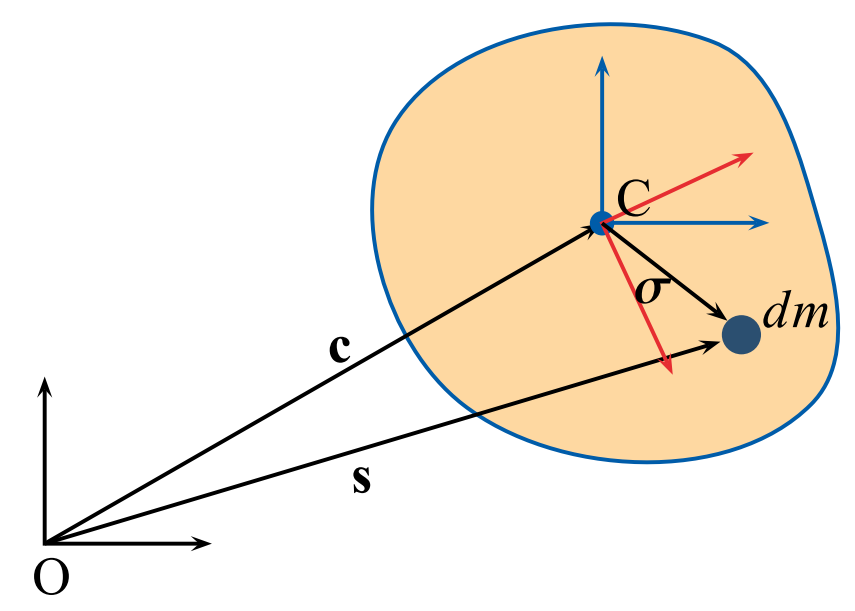
\includegraphics[width=0.3\textwidth]{images/Solide.PNG} \end{center}
\begin{align*}
\textbf{H}_C &= \int \boldsymbol{\sigma} \wedge \dot{\boldsymbol{\sigma}} \; d m \\
&= \int \boldsymbol{\sigma} \wedge ( \textbf{w} \wedge \boldsymbol{\sigma} ) \; d m \qquad \qquad \textbf{a} \wedge (\textbf{b} \wedge \textbf{c}) = \textbf{b} (\textbf{a} \cdot \textbf{c}) - \textbf{c} (\textbf{a} \cdot \textbf{b}) \\
&= \int \textbf{w} \| \boldsymbol{\sigma} \|^2 - \boldsymbol{\sigma} (\boldsymbol{\sigma} \cdot \textbf{w}) \; d m \\
&= \int ( \| \boldsymbol{\sigma} \|^2 \textbf{I} - \boldsymbol{\sigma} \; \boldsymbol{\sigma} ) \cdot \textbf{w} \; d m = \textbf{w} \cdot \int ( \| \boldsymbol{\sigma} \|^2 \textbf{I} - \boldsymbol{\sigma} \; \boldsymbol{\sigma} ) \; d m \\
&= \textbf{J}_C \cdot \textbf{w} \qquad \qquad \text{ où } \textbf{J}_C = \int ( \| \boldsymbol{\sigma} \|^2 \textbf{I} - \boldsymbol{\sigma} \; \boldsymbol{\sigma} ) \; d m
\end{align*}





%% Tenseur identité
\item Le tenseur identité \textbf{I} est : 
\[ \textbf{I} = \underline{\underline{I}} = \begin{pmatrix} 1 & 0 & 0 \\ 0 & 1 & 0 \\ 0 & 0 & 1 \\ \end{pmatrix} = \textbf{e}_1 \; \textbf{e}_1 + \textbf{e}_2 \; \textbf{e}_2 + \textbf{e}_3 \; \textbf{e}_3 = \begin{pmatrix} 1 & 0 & 0 \\ 0 & 0 & 0 \\ 0 & 0 & 0 \\ \end{pmatrix} + \begin{pmatrix} 0 & 0 & 0 \\ 0 & 1 & 0 \\ 0 & 0 & 0 \\ \end{pmatrix} + \begin{pmatrix} 0 & 0 & 0 \\ 0 & 0 & 0 \\ 0 & 0 & 1 \\ \end{pmatrix} \]
tel que : $\displaystyle \textbf{I} \; \textbf{a} = \textbf{a} $, et ce pour tout \textbf{a} de dimensions correspondantes (que \textbf{a} soit un vecteur ou un tenseur).





%% Tenseur central d'inertie
\item Le tenseur central d'inertie $\displaystyle \textbf{J}_C = \int (\| \textbf{s} \|^2 \textbf{I} - \textbf{s} \; \textbf{s}) \; d m $ peut être représenté par une matrice symétrique : 
\[ \begin{pmatrix} J_x & - J_{x y} & - J_{x z} \\ - J_{x y} & J_{y} & - J_{y z} \\ - J_{x z} & - J_{y z} & J_{z} \end{pmatrix} = \int \begin{pmatrix} y^2 + z^2 & - x y & - x z \\ - x y & x^2 + z^2 & - y z \\ - x z & - y z & x^2 + y^2 \end{pmatrix} \; d m \]
car $ \textbf{s} = x \; \textbf{e}_x  + y \; \textbf{e}_y + z \; \textbf{e}_z $. \\
On peut mettre cette matrice sous forme diagonale, les éléments de cette diagonale sont appelés \emph{moments principaux d'inertie} et les axes correspondants \emph{axes principaux d'inertie}.





%% Repère de König
\item Un repère de König est un repère non-inertiel de centre C dont les axes sont constamment parallèles aux axes d'un repère inertiel.
\begin{center} \begin{tikzpicture}
\coordinate (c) at (4,-1.5);
\draw [red,rounded corners=1mm] (c) \irregularcircle{1.5cm}{1mm};

    \draw [->, thick] node[above left]{O} (0,0,0) -- (1,0,0);
    \draw [->, thick] (0,0,0) -- (0,1,0);
    \draw [->, thick] (0,0,0) -- (0,0,1);

    \draw [->, thick] (c) node[above left]{C} -- ($ (c) + (1,0,0) $);
    \draw [->, thick] (c) -- ($ (c) + (0,1,0) $);
    \draw [->, thick] (c) -- ($ (c) + (0,0,1) $);

\node (Koenig) [xshift = 8cm, yshift = 0cm] {Repère de König};
\draw [->, thin] (Koenig.south west) -- ($ (c) + (0.1,0.1) $);
\end{tikzpicture} \end{center}





%% Ellipsoïde d'inertie
\item Ellipsoïde d'inertie : \\
Le moment d'inertie autour d'une droite \emph{d} passant par \emph{C} est donné par : $\displaystyle J_d = \int x^2 \; d m > 0 $ (sauf si la masse est sur l'axe). \\
Soit $ \boldsymbol{\omega} = \omega \; \textbf{e} $ (vecteur de Poisson) avec $ \| \textbf{e} \| = 1 $, on a : 
\[ T_C = \frac{1}{2} \boldsymbol{\omega} \cdot\textbf{J}_C \cdot \boldsymbol{\omega} = \frac{1}{2} \omega^2 \textbf{e} \cdot \textbf{J}_C \cdot \textbf{e} = \frac{1}{2} \omega^2 \; J_d \]
Si on fait varier le vecteur \textbf{e} (on le fait tourner autour de \emph{C}), on reporte le vecteur $\displaystyle \textbf{q} = \frac{1}{\sqrt{J}} \textbf{e} $. On obtient un ellipsoïde d'inertie $\displaystyle \Big( \textbf{q} \cdot \textbf{J}_C \cdot \textbf{q} = \frac{\textbf{e} \cdot \textbf{J}_C \cdot \textbf{e}}{J_d} = \frac{J_d}{J_d} = 1 \Big) $.

\begin{center} \begin{tabular}{p{5cm}p{5cm}}
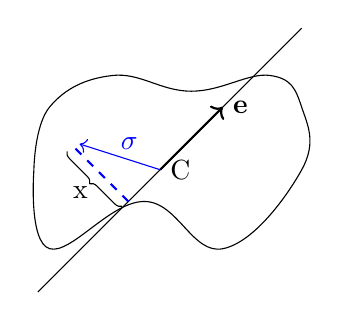
\begin{tikzpicture}
\draw  plot[smooth, tension=.7, scale=0.4] coordinates {(-3.5,0.5) (-3,2.5) (-1,3.5) (1.5,3) (4,3.5) (5,2.5) (5,0.5) (2.5,-2) (0,-0.5) (-3,-2) (-3.5,0.5)};
\draw [-] (-1.35,-1.35) -- (2,2);
\draw [->, thick] (0.203,0.203) node[right]{C} -- (1,1) node[right]{\textbf{e}};
\draw [-, dashed, draw=blue, thick] (-0.2,-0.2) -- (-0.907,0.507);
\draw [decorate,decoration={brace,raise=0.1cm}] (-0.21,-0.19) -- (-0.907,0.507) node[midway, xshift = -0.25cm, yshift = -0.25cm]{x};
\draw [->, draw = blue] (0.203,0.203) -- (-0.82,0.53) node[right, xshift=0.4cm]{\color{blue} $ \sigma $};
\end{tikzpicture}
&
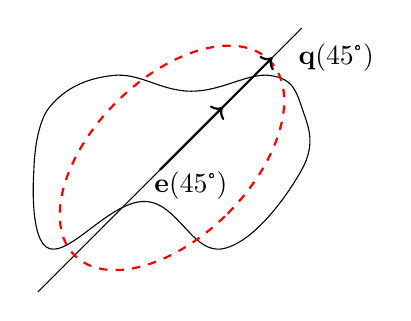
\begin{tikzpicture}
\draw  plot[smooth, tension=.7, scale=0.4] coordinates {(-3.5,0.5) (-3,2.5) (-1,3.5) (1.5,3) (4,3.5) (5,2.5) (5,0.5) (2.5,-2) (0,-0.5) (-3,-2) (-3.5,0.5)};
\draw [-] (-1.35,-1.35) -- (2,2);
\draw[rotate=-45, draw=red, dashed, thick] (0,0.5) ellipse (1cm and 1.75cm);
\draw [->, thick] node[right, yshift=0cm]{\textbf{e}(45°)} (0.203,0.203) -- (1,1);
\draw [->, thick] (0.203,0.203) -- (1.63,1.63) node[right, xshift=0.2cm]{\textbf{q}(45°)};

\end{tikzpicture}
\end{tabular} \end{center}





%% Théorème de transport
\item Théorème de transport : 
\begin{align*}
J_d' &= \textbf{e} \cdot \textbf{J}_O \cdot \textbf{e} = \textbf{e} \cdot \bigg( m \Big[ \| \textbf{c} \|^2 \textbf{I} - \textbf{c \textbf{c}} \Big] + \textbf{J}_C \bigg) \cdot \textbf{e} \\
&= m \; l^2 + J_d
\end{align*}

\begin{center} 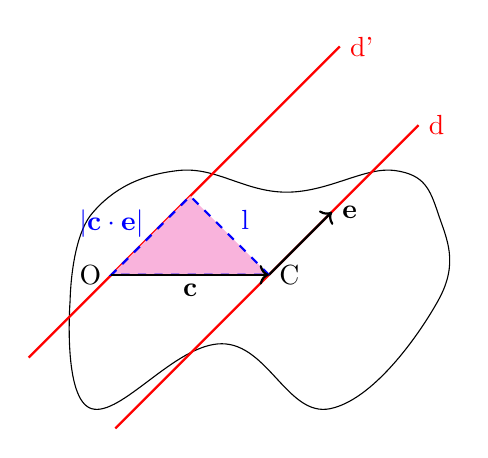
\begin{tikzpicture}
\draw  plot[smooth, tension=.7, scale=0.55] coordinates {(-3.5,0.5) (-3,2.5) (-1,3.5) (1.5,3) (4,3.5) (5,2.5) (5,0.5) (2.5,-2) (0,-0.5) (-3,-2) (-3.5,0.5)};
\draw [-, red, thick] (-1.35,-1.35) -- (2.5,2.5) node[right]{d};
\draw [-, red, thick] (-2.45,-0.45) -- (1.5,3.5) node[right]{d'};
\draw [->, thick] (0.6,0.6) -- (1.4,1.4) node[right]{\textbf{e}};

\draw [fill=magenta!30, draw=blue, dashed, thick]  (0.6,0.6) node[right]{C} -- node[midway, xshift=0.2cm, yshift=0.2cm]{\color{blue} l} (-0.4,1.6) -- node[midway, xshift=-0.5cm, yshift=0.15cm]{\color{blue} $|\textbf{c} \cdot \textbf{e}|$} (-1.4,0.6) node[left]{O} -- cycle;
\draw [->, thick] (-1.4,0.6) -- (0.6,0.6) node[midway, yshift=-0.2cm]{\textbf{c}};
\end{tikzpicture} \end{center}





%% Mouvement relatif de deux solides
\item Mouvement relatif de deux solides : 
\begin{center}
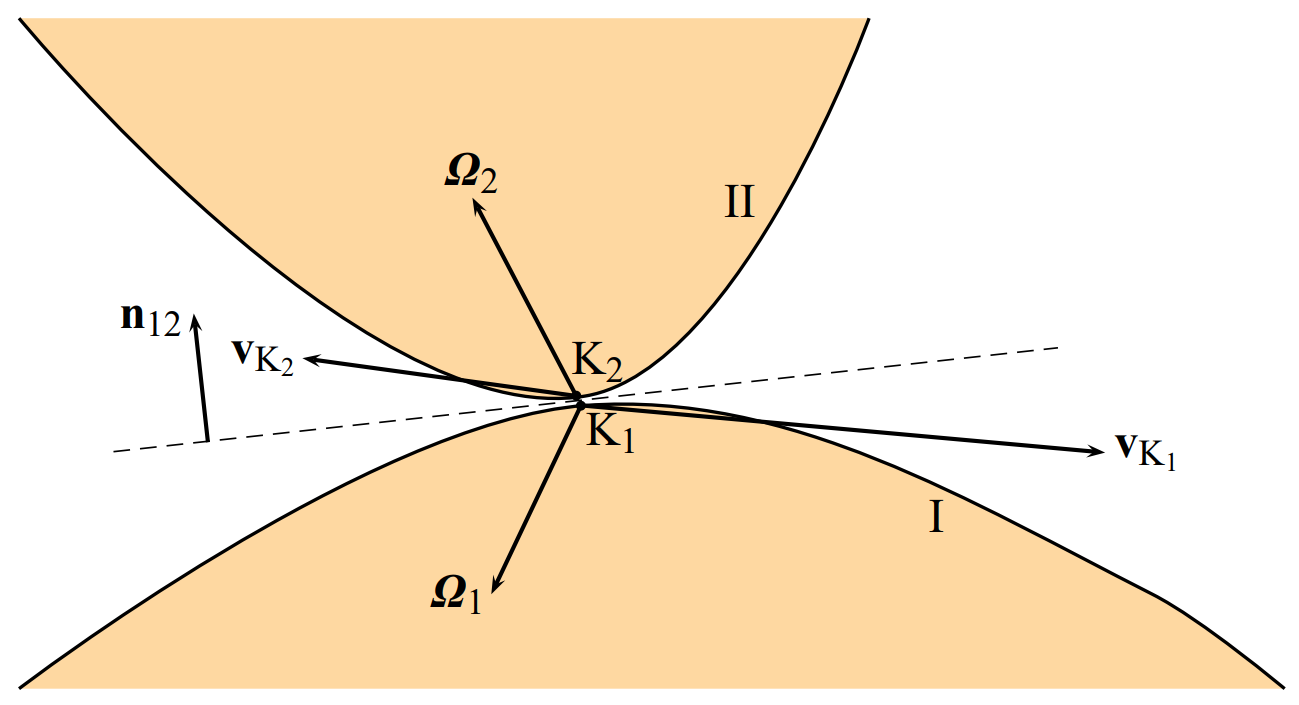
\includegraphics[width=0.5\textwidth]{images/Solides.PNG}
\end{center}
\begin{itemize}
\item Solide I : $ \textbf{v}_{K_1}, \; \boldsymbol{\Omega}_1 $
\item Solide II : $ \textbf{v}_{K_2}, \; \boldsymbol{\Omega}_2 $
\end{itemize}
Mouvement relatif de II par rapport à I : 
\begin{itemize}
\item Vitesse de glissement : $ \textbf{v}_{21} = \textbf{v}_{K_2} - \textbf{v}_{K_2} $
\item Vitesse relative de rotation : $ \boldsymbol{\Omega}_{21} = \boldsymbol{\Omega}_2 - \boldsymbol{\Omega}_1 $
\end{itemize}
Glissement : 
\begin{center}
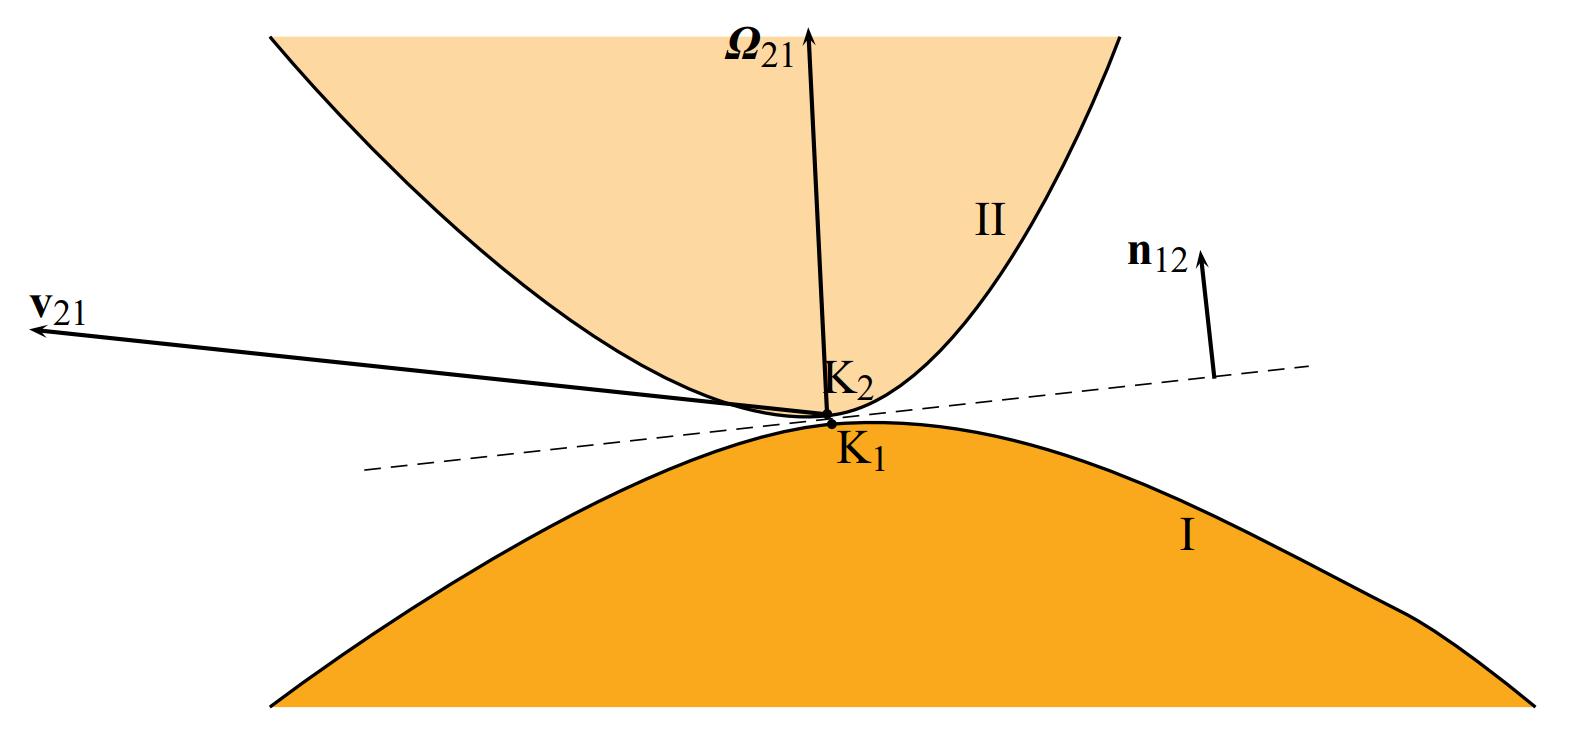
\includegraphics[width=0.5\textwidth]{images/Solides2.PNG}
\end{center}
\begin{itemize}
\item Pas d’interpénétration des deux solides : $ \textbf{v}_{21} \cdot \textbf{n}_{12} \geq 0 $.
\item Roulement (avec glissement) : $ \textbf{v}_{21} \cdot \textbf{n}_{12} = 0 $
\item Roulement sans glissement : $ \textbf{v}_{21} = \textbf{0} $, i.e. $ \textbf{v}_{K_2} = \textbf{v}_{K_1} $.
\end{itemize}
Roulement sans glissement : 
\begin{center}
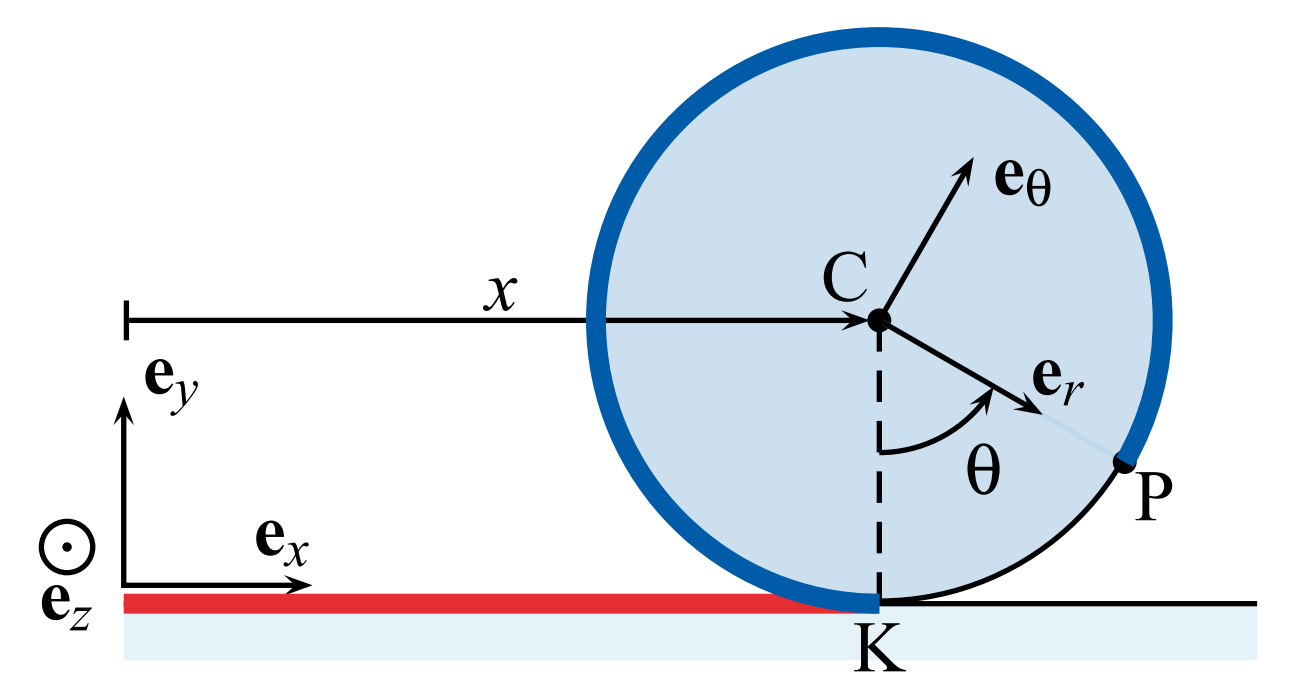
\includegraphics[width=0.5\textwidth]{images/Solides3.PNG}
\end{center}
\begin{align*}
\textbf{s}_p &= x \textbf{e}_x + R \textbf{e}_y + R \textbf{e}_r \\
\dot{\textbf{s}}_p &= \dot{x} \textbf{e}_x + R \dot{\theta} \textbf{e}_\theta
\end{align*}
\[ \fbox{$ \; \dot{x} + R \dot{\theta} = 0 \; $} \]





\end{itemize}




















\section{Théorie : Lois de la dynamique newtonienne}










\begin{itemize}





%% Axiomes de la dynamique newtonienne
\item Axiomes de la dynamique newtonienne : 
\begin{enumerate}
\item Le temps est une grandeur absolue indépendante de tout système de référence.
\item Les masses sont des constantes positives (ou nulles) additives.
\item Les fonctions $ \textbf{s}(t) $ sont continûment dérivables et deux fois continûment dérivables par morceaux.
\item Les forces satisfont au principe de l'action et de la réaction selon lequel les forces que deux éléments matériels distincts exercent l'un sur l'autre sont égales en norme, de signes opposés et parallèles à la droite joignant ces deux éléments.
\end{enumerate}





%% Repère inertiel
\item Dans un repère inertiel, un corps isolé de toute interaction avec le monde extérieur ne peut être qu'au repos ou en MRU (première loi de Newton ou principe d'inertie).





%% Loi fondamentale de la dynamique newtonienne
\item Lorsqu'un corps est soumis à des forces, on admet la loi suivante (loi fondamentale de la dynamique newtonienne) : 
\begin{center}
\ovalbox {\begin{minipage}{0.93\textwidth}
Dans un repère inertiel, la résultante des forces appliquées à un point matériel (ou à un élément matériel infinitésimal) est égale à la dérivée temporelle de sa quantité de mouvement : 
\[ \textbf{G} = \frac{d \textbf{N}_O}{d t} = \frac{d}{d t} (m \; \dot{\textbf{s}}) \]
\end{minipage}}
\end{center}





%% Théorème de la quantité de mouvement
\item Théorème de la quantité de mouvement : 
\begin{center}
\ovalbox {\begin{minipage}{0.93\textwidth}
Dans un repère inertiel, la dérivée temporelle de la quantité de mouvement d'un système matériel est égale à la résultante des forces extérieures qui lui sont appliquées : 
\[ \frac{d \textbf{N}_O}{d t} = \textbf{G} \]
\end{minipage}}
\end{center}
Ce qui implique que le centre d'inertie d'un système (de masse m) "agit" comme un point matériel de masse m soumis à la résultante des forces extérieures ($ m \; \ddot{\textbf{c}} = \textbf{G} $).





%% Théorème du moment cinétique
\item Théorème du moment cinétique : 
\begin{center}
\ovalbox {\begin{minipage}{0.93\textwidth}
Dans un repère inertiel, la dérivée temporelle du moment cinétique d'un système matériel par rapport à un point fixe O est égale à la résultant des moments par rapport à ce point des forces extérieures appliquées au système : 
\[ \dot{\textbf{H}}_O = \textbf{M}_O \]
\end{minipage}}
\end{center}





%% Théorème de l'énergie cinétique
\item Théorème de l'énergie cinétique : 
\begin{center}
\ovalbox {\begin{minipage}{0.93\textwidth}
Dans un repère inertiel, la puissance développée par l'ensemble des forces intérieures appliquées à un système matériel est égale à la dérivée temporelle de son énergie cinétique : 
\[ \dot{T}_O = \mathpzc{P}_O \]
\end{minipage}}
\end{center}





%% Statique
\item En l'absence de tout mouvement (statique), on a : $\displaystyle \textbf{G} = \textbf{0} \qquad \textbf{M}_O = \textbf{0} $.





%% Théorème généraux
\item Les trois théorèmes précédents sont aussi appelés théorèmes généraux et peuvent s'écrire sous formes intégrales : 
\begin{enumerate}
\item $\displaystyle \textbf{N}_O(t_2) - \textbf{N}_O(t_1) = \int_{t_1}^{t_2} \textbf{G}(t) \; d t $
\item $\displaystyle \textbf{H}_O(t_2) - \textbf{H}_O(t_1) = \int_{t_1}^{t_2} \textbf{M}_O(t) \; d t $
\item $\displaystyle T_O(t_2) - T_O(t_1) = \int_{t_1}^{t_2} \mathpzc{P}_O(t) \; d t $
\end{enumerate}





%% Théorèmes généraux dans un repère non-inertiel
\item Voici les théorèmes généraux dans un repère non-inertiel : 
\begin{enumerate}
\item Première loi de Newton : $\displaystyle m \; \textbf{a}_r = m \frac{\delta^2 \textbf{r}}{\delta t^2} = \textbf{G} - m \; \textbf{a}_e - m \; \textbf{a}_c $.
\item Quantité de mouvement : $\displaystyle \frac{\delta \textbf{N}_{O'}}{\delta t} = \textbf{G} + \textbf{F}_e + \textbf{F}_c $.
\item Moment cinétique : $\displaystyle \dot{\textbf{H}}_B = \frac{\delta \textbf{H}_B}{\delta t} = \textbf{M}_B - m \; (\textbf{c} - \textbf{b}) \wedge \ddot{\textbf{b}} $.
\item Énergie cinétique : $\displaystyle \dot{T}_B = \mathpzc{P} - m \; (\dot{\textbf{c}} - \dot{\textbf{b}}) \cdot \ddot{\textbf{b}} $.
\end{enumerate}





%% Système à masse variable
\item Dans un système à masse variable, la loi fondamentale de Newton ($\displaystyle \textbf{F} = m \; \textbf{a} $) s'écrit : 
\[ \frac{d}{d t} (m \textbf{v}) = m \frac{d \textbf{v}}{d t} + \frac{d m}{d t} \textbf{v} = \textbf{G} \]
si et seulement si $\displaystyle \textbf{P} = - \frac{d m}{d t} \textbf{v} $ où \textbf{P} est une force accélératrice dite de "poussée", ce qui nous donne : $\displaystyle m \frac{d \textbf{v}}{d t} = \textbf{G} + \textbf{P} $.







\end{itemize}





















\section{Théorie : Modélisation et analyse des systèmes mécaniques}











\begin{itemize}






%% Variables adimensionnelles
\item Toutes les grandeurs physiques utilisées en mécanique peuvent être exprimées à partir des trois grandeurs fondamentales : L la longueur, T le temps et M la masse. \\
Pour une grandeur X quelconque, on a $\displaystyle [X] = L^{\alpha} \; T^{\beta} \; M^{\gamma} $ et si X est adimensionnel, alors $\displaystyle [X] = 1 $.





%% Théorème pi
\item Le théorème $ pi $ (ou théorème de Vaschy-Buckingham) affirme que le nombre de produits sans dimension indépendants qui peuvent être construits à partir de n grandeurs physiques est égal à $ n - N $ où N désigne le nombre de grandeurs fondamentales intervenant dans la mesure des n grandeurs.





%% Intégrales premières du mouvement d'un système
\item Lorsque la projection sur un axe fixe \textbf{e} de la \emph{résultante} ou du \emph{moment résultant} des forces extérieures appliquées à un système matériel est nulle, on obtient immédiatement une intégrale première du mouvement de ce système. On a en effet, en vertu du théorème de la quantité de mouvement ou du théorème du moment cinétique exprimé dans un repère inertiel ou un système d'axes centrés au centre d'inertie du système et constamment parallèles à des axes inertiaux ($ \implies $ vecteur de Poisson $ = 0 $), 
\begin{align*}
\textbf{e} \cdot \dot{\textbf{N}}_O = \textbf{e} \cdot \textbf{G} &= 0 &&\implies &\textbf{e} \cdot \textbf{N}_O &= \text{ constante } \\
\textbf{e} \cdot \dot{\textbf{H}}_O = \textbf{e} \cdot \textbf{M}_O &= 0 &&\implies &\textbf{e} \cdot \textbf{H}_O &= \text{ constante } \\
\textbf{e} \cdot \dot{\textbf{H}}_C = \textbf{e} \cdot \textbf{M}_C &= 0 &&\implies &\textbf{e} \cdot \textbf{H}_C &= \text{ constante } \\
\end{align*}





%% Intégrales premières - Forces conservatives
\item Lorsque les forces appliquées à un système sont conservatives ou ne développent pas de puissance dans un repère inertiel, il vient : 
\[ \frac{d T_O}{d t} = \mathpzc{P}_O = - \frac{d V}{d t} \qquad \implies \qquad T_O + V = E = \text{ constante } \]





%% Intégrale première - Loi de Newton
\item Dans le cas de l'étude du mouvement d'un point matériel, le théorème de l'énergie cinétique est une conséquence directe de la loi fondamentale de Newton. L'intégrale première de conservation de l'énergie peut donc être obtenue également directement à partir de la loi de Newton. \\
Exemple : 
\begin{itemize}
    \item Glissement sans frottement sur un courbe/surface. \\
    On multiplie l'équation de Newton scalairement par $ \dot{\textbf{s}} $. Et on obtient : 
    \begin{align*} m \ddot{\textbf{s}} &= \textbf{G} + \textbf{R} &m \dot{\textbf{s}} \cdot \ddot{\textbf{s}} &= \dot{\textbf{s}} \cdot (\textbf{G} + \textbf{R}) = \dot{\textbf{s}} \cdot \textbf{G} \end{align*}
    Si les forces données dérivent d'un potentiel, on a : $\displaystyle \dot{\textbf{s}} \cdot \textbf{G} = - \frac{d V}{d t} $. \\
    Et l'intégrale première de conservation de l'énergie : $\displaystyle \frac{1}{2} m \| \dot{\textbf{s}} \|^2 + V = E $. \\
    Cette façon de procéder est assez générale et permet d'obtenir des intégrales premières qui n'apparaissent pas directement par application des théorèmes généraux.

    \item Mouvement d'un point matériel sur une courbe/surface de guidage mobile.
    \begin{align*} m \frac{d^2 \textbf{s}}{d t^2} &= \textbf{G} + \textbf{R} &m \frac{\delta \textbf{s}}{\delta t} \cdot \frac{d^2 \textbf{s}}{d t^2} = \frac{\delta \textbf{s}}{\delta t} \cdot (\textbf{G} + \textbf{R}) &= \frac{\delta \textbf{s}}{\delta t} \cdot \textbf{G} \end{align*}
    Cette fois-ci, on a multiplié l'équation scalairement par la dérivée relative du point par rapport à la courbe/surface. Dans certains cas, cette équation donne lieu à une intégrale première de bilan énergétique. Dans tous les cas, l'intégrale de : $\displaystyle \frac{\delta \textbf{s}}{\delta t} \cdot \textbf{G} $ joue le rôle de potentiel et la constante d'intégration représente une certaine forme de conservation d'énergie du système.
\end{itemize}





%% Diagramme de potentiel
\item À partir de l'intégrale première du mouvement exprimant la conservation de l'énergie totale d'un système mécanique décrite précédemment, on va tracer un diagramme de potentiel. Puisque l'énergie cinétique $ T_O > 0 $, on peut écrire : 
\[ T_O = E - V \geq 0 \]
On en déduit que les seules configurations accessibles sont telles que : $ V(\textbf{s}) \leq 0 $. Le graphique de $ V(q) $, où \emph{q} est la variable du système, est appelé diagramme de potentiel.





%% Positions d'équilibre
\item Les positions d'équilibre d'un système sont caractérisées par une accélération et une vitesse nulle. Pour trouver les position d'équilibre, on pose donc $ \ddot{x} = 0 $ et $ \dot{x} = 0 $ dans l'équation du mouvement, où \emph{x} est la variable caractéristique du système.





%% Méthode des perturbations infinitésimales
\item Pour la méthode des perturbations infinitésimales, on utilise l'équation : 
\[ \ddot{x} + F(x) = 0 \]
(équation de Newton) dans laquelle on introduit : 
\[ x = x_{\text{eq}} + \upeta \]
où $ x_{\text{eq}} $ est la position d'équilibre et $ \upeta $ est la perturbation. \\
L'équation devient : 
\[ ( \underbrace{\ddot{x}_{\text{eq}}}_{0} + \; \ddot{\upeta} \; ) + F(x_{\text{eq}} + \upeta) = 0 \]
Et pour $ F(x_{\text{eq}} + \upeta) $, on va faire le développement de Taylor au voisinage de $ x_{\text{eq}} $ à l'ordre 1. \\
L'équation devient donc : 
\[ \ddot{\upeta} + \underbrace{F(x_{\text{eq}})}_{0} + F'(x_{\text{eq}}) \; (\underbrace{x - x_{\text{eq}}}_{\upeta}) = 0 \]
\[ \implies \qquad \ddot{\upeta} + F'(x_{\text{eq}}) \upeta = 0 \qquad \text{ Équation linéaire } \]
On étudie dés lors la stabilité en fonction de la résolution de l'équation différentielle ci-dessus. \\
Exemple : 
\begin{itemize}
\item Si $ F'(x_{\text{eq}}) = 0 $, alors $ \ddot{\upeta} = 0 $ et $ \upeta = A t + B \longrightarrow $ Équilibre faiblement stable
\item Si $ F'(x_{\text{eq}}) > 0 $, alors $ \upeta = A \cos \Big( \sqrt{F'(x_{\text{eq}})} \Big) + B \sin \Big( \sqrt{F'(x_{\text{eq}})} \Big) \longrightarrow $ Équilibre marginalement stable
\item Si $ F'(x_{\text{eq}}) < 0 $, alors $ \upeta = A \text{ ch } \Big( \sqrt{F'(x_{\text{eq}})} \Big) + B \text{ sh } \Big( \sqrt{F'(x_{\text{eq}})} \Big) \longrightarrow $ Équilibre instable
\end{itemize}
Remarque : $ F'(x_{\text{eq}}) = $ constante.





%% Stabilité des solutions de la méthode des perturbations infinitésimales
\item D'un point de vue plus général, la linéarisation de la dynamique des perturbations (infinitésimales) donne une équation linéaire à coefficients constants. Sa solution s'exprime sous la forme d'une somme d'expressions de la forme : 
\[ t^k \; e^{z t} \qquad \text{ avec \emph{k} entier $ \geq 0 $ } \]
où les \emph{z} sont les racines de l'équation caractéristique associée. \\
Ces expressions sont des fonctions croissantes en fonction du temps si la partie réelle de l'argument de l'exponentielle est positive et des fonctions décroissantes si cette partie réelle est négative. Il s'ensuit que : 
\begin{itemize}
\item Si toutes les racines ont une partie réelle négative, l'équilibre est stable.
\item Si une racine au moins a sa partie réelle positive, l'équilibre est instable.
\item Si toutes les racines ont une partie réelle négative sauf certaines qui ont une partie réelle nulle, les solutions élémentaires correspondantes sont des fonctions périodiques ($ k = 0 $) ou des fonctions croissantes en puissance de $ t $ ($ k > 0 $). Dans le premier cas, la perturbation est bornée mais pas amortie. On dit que l'équilibre est marginalement stable. Dans le second cas, la perturbation croît sans être cependant exponentiellement amplifiée. On dit que l'équilibre est faiblement instable au sens de l'analyse linéaire de la stabilité.
\end{itemize}
C'est grâce à la méthode des petites perturbations que l'on va analyser les positions d'équilibre marginalement stable et faiblement instables. Et lever le voile sur leurs réelle stabilité.

\begin{center} \begin{tabular}{|p{5cm}|p{5cm}|}
\hline
Polynôme caractéristique & Solution générale \\
\hline
$ \begin{aligned} &z^2 - \alpha^2 = 0 \implies \\ &z_1 = \alpha \; \; \& \; \; z_2 = - \alpha \end{aligned} $ & $ \begin{aligned} x(t) &= C'_1 e^{\alpha t} + C'_2 e^{- \alpha t} \\ &= C_1 \text{ sh } \alpha t + C_2 \text{ ch } \alpha t \end{aligned} $ \\
\hdashline
$ \begin{aligned} &z^2 + \alpha^2 = 0 \implies \\ &z_1 = i \alpha \; \; \& \; \; z_2 = - i \alpha \end{aligned} $ & $ \begin{aligned} x(t) &= C'_1 e^{i \alpha t} + C'_2 e^{- i \alpha t} \\ &= C_1 \sin \alpha t + C_2 \cos \alpha t \end{aligned} $ \\
\hdashline
$ \begin{aligned} z^2 &= 0 \implies \\ z_1 &= z_2 = 0 \end{aligned} $ & $ x(t) = A t + B $ \\
\hline
\end{tabular} \end{center}

\begin{center} \begin{tabular}{|p{6cm}|p{6cm}|}
\hline
Racines du polynôme caractéristique : $ z_1 = a_1 + i b_1 \; \; \& \; \; z_2 = a_2 + i b_2 $ & Stabilité : méthode des perturbations infinitésimales \\
\hline
$ a_1 < 0 $ et $ a_2 < 0 $ & Équilibre stable \\
\hdashline
Si $ a_1 > 0 $ ou $ a_2 > 0 $ & Équilibre instable \\
\hdashline
$ a_1 < 0 \; \& \; a_2 = 0 $ \; ou \; $ a_1 = 0 \; \& \; a_2 < 0  $ \; \danger avec $ k = 0 $ \quad (k = multiplicité) & Équilibre marginalement stable \\
\hdashline
$ z_1 = z_2 = 0 $ \qquad ($ k \neq 0 $) & Équilibre faiblement instable \\
\hline
\end{tabular} \end{center}
Exemple d'équilibre marginalement stable : $ x(t) = C'_1 e^{i \alpha t} + C'_2 e^{- i \alpha t} \; = C_1 \sin \alpha t + C_2 \cos \alpha t $.





%% Méthode des petites perturbations
\item Pour la méthode des petites perturbations, on commence en faisant comme pour la méthode des perturbations infinitésimales mais quand on a l'équation : 
\[ \ddot{\upeta} + F(x_{\text{eq}} + \upeta) = 0 \]
On doit faire le développement de Taylor et on ne s'arrête que lorsque l'on a un terme non nul. \\
Si $ F'(x_{\text{eq}}) \neq 0 $, la méthode des petites perturbations est différente de la méthode des perturbations infinitésimales. Sinon $ \big( F(x_{\text{eq}}) = 0 \big) $, elles sont exactement les mêmes. \\
Exemple : 
\[ \text{Si} \quad F'(x_{\text{eq}}) = 0 \; ; \; F^{(2)}(x_{\text{eq}}) = 0 \; ; \; F^{(3)}(x_{\text{eq}}) = 0 \; ; \; F^{(4)}(x_{\text{eq}}) \neq 0 \]
\[ \text{alors} \quad \ddot{\upeta} + \underbrace{ F(x_{\text{eq}}) + F'(x_{\text{eq}}) \upeta + F^{(2)}(x_{\text{eq}}) \frac{\upeta^2}{2 !} + ... \; + }_{0} F^{(4)}(x_{\text{eq}}) \frac{\upeta^4}{4 !} = 0 \]
\[ \implies \quad \ddot{\upeta} + \underbrace{\frac{F^{(4)}(x_{\text{eq}})}{4 !}}_{\text{constant}} \upeta^4 = 0 \]
On n'a donc plus une équation différentielle \emph{linéaire} même si les coefficients sont toujours constants. \\
Pour pouvoir obtenir une intégrale première, on va multiplier cette équation par $ \dot{\upeta} $. \\
On étudie ensuite la stabilité de l'équilibre à partir de cette intégrale première. \\
L'équilibre est stable si $ \upeta $, qui est la perturbation, diminue ou reste constant. Sinon, l'équilibre est instable.





%% Stabilité des solutions de la méthode des petites perturbations
\item De manière plus générale, considérons un système à un degré de liberté dont la dynamique des petites perturbations est décrite par l'équation : 
\[ \ddot{\upeta} + \mu \; \upeta^k = 0 \]
où \emph{k} est un naturel non nul et $ \mu $ désigne une constante quelconque. Multipliant par $ \dot{\upeta} $ et intégrant terme à terme, il vient : 
\[ \frac{1}{2} \dot{\upeta}^2 + \frac{\mu}{k + 1} \upeta^{k + 1} = \text{ constante } \]
Même si on ne sait pas résoudre complètement l'équation différentielle, l'intégrale première permet de conclure quant à la stabilité de la position d'équilibre : 
\begin{itemize}
\item Si \emph{k} est impair et $ \mu $ positif, le membre de gauche de l'intégrale première $\displaystyle \Big( \frac{1}{2} \dot{\upeta}^2 + \frac{\mu}{k + 1} \upeta^{k + 1} \Big) $ est une somme bornée de deux carrés. Chacun des termes est donc borné et l'équilibre est stable.
\item Si \emph{k} est impair et $ \mu $ négatif, l'intégrale première exprime que la différence des deux termes positifs du membre de gauche reste constante mais permet à ces deux termes de prendre des valeurs arbitrairement grandes. La perturbation n'est donc pas bornée et l'équilibre est instable.
\item Si \emph{k} est pair, quel que soit $ \mu $ il existe toujours une évolution de la perturbation qui n'est pas bornée. L'équilibre est instable.
\end{itemize}

\begin{center} \begin{tabular}{|p{6cm}|p{6cm}|}
\hline
$\displaystyle \frac{1}{2} \dot{\upeta}^2 + \frac{\mu}{k + 1} \upeta^{k + 1} = \text{ constante } $ & Stabilité : méthode des petites perturbations \\
\hline
\emph{k} impair \; \& \; $ \mu $ positif & Équilibre stable \\
\hdashline
\emph{k} impair \; \& \; $ \mu $ négatif & Équilibre instable \\
\hdashline
\emph{k} pair & Équilibre instable \\
\hline
\end{tabular} \end{center}





%% Point stationnaire et diagramme de potentiel
\item Dans le cas où le système est décrit par une intégrale première du type : 
\[ \frac{1}{2} m \dot{x}^2 + V(x) = E \]
ou par toute autre intégrale de même structure, la stabilité peut être discutée directement à partir de l'étude des variations de $ V(x) $. \\
L'équation de mouvement correspondant à cette équation s'obtient par dérivation : 
\[ m \ddot{x} + V'(x) = 0 \]
Les éventuelles positions d'équilibre $ x_{\text{eq}} $ sont données par : $ V'(x_{\text{eq}}) = 0 $, et correspondent aux \emph{points stationnaires} du potentiel \emph{V}.





%% Stabilité et diagramme de potentiel
\item Pour caractériser une position d'équilibre, considérons une petite perturbation $ \upeta $ de celle-ci selon : 
\[ x = x_{\text{eq}} + \upeta \qquad \qquad \dot{x} = \dot{\upeta} \qquad \qquad \ddot{x} = \ddot{\upeta} \]
La perturbation obéit à l'équation : 
\[ m \ddot{\upeta} + V'(x_{\text{eq}} + \upeta) = 0 \]
En limitant au premier terme non nul le développement en série de Taylor de $ V'(x) $ au voisinage de $ x = x_{\text{eq}} $, on obtient l'équation approchée : 
\[ m \ddot{\upeta} + \frac{1}{k !} V^{(k+1)} (x_{\text{eq}}) \upeta^k \]
qui est similaire à l'équation obtenue dans l'étude des petites perturbations $\displaystyle \Big( \frac{1}{2} \dot{\upeta}^2 + \frac{\mu}{k + 1} \upeta^{k + 1} = \text{ constante} \Big) $ avec $\displaystyle \mu = \frac{1}{m \; k !} V^{(k + 1)} (x_{\text{eq}}) $. \\
En s'appuyant sur les résultats dégagés dans l'étude des petites perturbations, on en déduit la stabilité de l'équilibre : 
\begin{itemize}
\item Si \emph{k} est impair et $ \mu $ positif, c'est-à-dire si la première dérivée non-nulle du potentiel en $ x_{\text{eq}} $ est d'ordre pair et que la valeur de celle-ci est positive, l'équilibre est stable. Cette condition correspond à l'existence d'un minimum local du potentiel en $ x_{\text{eq}} $.
\item Si \emph{k} est impair et $ \mu $ négatif, c'est-à-dire si la première dérivée non-nulle du potentiel en $ x_{\text{eq}} $ est d'ordre pair et que la valeur de celle-ci est négative, l'équilibre est instable. Cette situation se produit en tout maximum local du potentiel.
\item Si \emph{k} est pair, quel que soit $ \mu $, c'est-à-dire si la première dérivée non-nulle du potentiel en $ x_{\text{eq}} $ est d'ordre impair, l'équilibre est instable. Le graphe du potentiel $ V(x) $ présente un point d'inflexion à tangente horizontale en un tel point.
\end{itemize}





%% Explications pratiques de l'utilisation du diagramme de potentiel
\item En pratique, on utilise le potentiel de la manière suivante : Pour trouver les positions d'équilibre, on peut aussi dériver le potentiel $ \big( \rightarrow V'(x) \big) $ et voir où ça s'annule. \\
Ensuite, on calcule la dérivée seconde pour voir si c'est stable : 
\begin{itemize}
\item $ V''(x) < 0 \longrightarrow $ \; 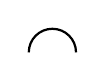
\begin{tikzpicture} \draw [-, thick] (-0.3,2.5) arc (180:0:.3cm); \end{tikzpicture} \; $ [ - x^2 \rightarrow f'' = - 2 ] $
\item $ V''(x) > 0 \longrightarrow $ \; 
\begin{tikzpicture} \draw [-, thick] (-0.3,2.5) arc (-180:0:.3cm); \end{tikzpicture} \; $ [ + x^2 \rightarrow f'' = + 2 ] $
\item $ V''(x) = 0 \longrightarrow $ Aucune information, il faut encore dériver.
\end{itemize}
\danger Il faut dériver $ V(x) $ en fonction de \emph{x} $\displaystyle \longrightarrow V'(x) = \frac{d V(x)}{d x} $.





%% Rappel : extrema d'une fonction
\item Rappel : Extrema d'une fonction : \\
Si \emph{f} est une fonction réelle $ n + 1 $ fois continûment dérivable sur $ ]a, b[ $, si $ f'(c) = 0 $ en un point $ c \in \; ]a, b[ $ et si la première dérivée non-nulle en \emph{c} est $ f^{(n)} (c) $, alors : 
\begin{itemize}
\item \emph{c} est un maximum local si \emph{n} est pair et $ f^{(n)}(c) < 0 $.
\item \emph{c} est un minimum local si \emph{n} est pair et $ f^{(n)}(c) > 0 $.
\item \emph{c} est un point d'inflexion à tangente horizontale si \emph{n} est pair.
\end{itemize}





%% Oscillateur amorti
\item L'oscillateur amorti  est constitué d'une masse, d'un ressort et d'un amortisseur. On note $ x(t) $ l'élongation du ressort par rapport à sa longueur naturelle $ l_0 $. L'équation de Newton donne : 
\[ m \; \ddot{x} = - c \; \dot{x} - k \; x \]

\begin{center}
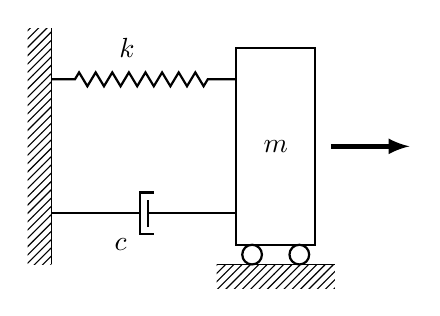
\begin{tikzpicture}[every node/.style={draw,outer sep=0pt,thick}]
\tikzstyle{spring}=[thick,decorate,decoration={zigzag,pre length=0.3cm,post length=0.3cm,segment length=6}]
\tikzstyle{damper}=[thick,decoration={markings,  
  mark connection node=dmp,
  mark=at position 0.5 with 
  {
    \node (dmp) [thick,inner sep=0pt,transform shape,rotate=-90,minimum width=15pt,minimum height=3pt,draw=none] {};
    \draw [thick] ($(dmp.north east)+(2pt,0)$) -- (dmp.south east) -- (dmp.south west) -- ($(dmp.north west)+(2pt,0)$);
    \draw [thick] ($(dmp.north)+(0,-5pt)$) -- ($(dmp.north)+(0,5pt)$);
  }
}, decorate]
\tikzstyle{ground}=[fill,pattern=north east lines,draw=none,minimum width=0.75cm,minimum height=0.3cm]



\begin{scope}[xshift=7cm]
\node (M) [minimum width=1cm, minimum height=2.5cm] {$m$};

\node (ground) [ground,anchor=north,yshift=-0.25cm,minimum width=1.5cm] at (M.south) {};
\draw (ground.north east) -- (ground.north west);
\draw [thick] (M.south west) ++ (0.2cm,-0.125cm) circle (0.125cm)  (M.south east) ++ (-0.2cm,-0.125cm) circle (0.125cm);

\node (wall) [ground, rotate=-90, minimum width=3cm,yshift=-3cm] {};
\draw (wall.north east) -- (wall.north west);

\draw [spring] (wall.170) -- ($(M.north west)!(wall.170)!(M.south west)$) node[pos=.5,left, draw=none, yshift = 0.4cm]{$k$};
\draw [damper] (wall.10) -- ($(M.north west)!(wall.10)!(M.south west)$) node[pos=.5,left, draw=none, yshift = -0.4cm, xshift = -0.1cm]{$c$};

\draw [-latex,ultra thick] (M.east) ++ (0.2cm,0) -- +(1cm,0);
\end{scope}
\end{tikzpicture}
\end{center}

où m la masse, c la constante d'amortissement, k la raideur du ressort sont des constantes positives. On pose $\displaystyle \omega_0 = \sqrt{\frac{k}{m}} $ appelée fréquence propre du système et $\displaystyle \zeta = \frac{c}{2 \sqrt{k \; m}} $ appelé facteur d'amortissement du système. Et on a donc l'équation de Newton sous forme canonique : 
\[ \ddot{x} + 2 \; \zeta \; \omega_0 \; \dot{x} + \omega_0^2 \; x = 0 \]

%   Explication => lignes sur les cotés

\begin{siderules}
En l'absence d'amortissement ($ c = 0 $), l'équation différentielle du mouvement devient : $\displaystyle \ddot{x} + \omega_0^2 \; x = 0 $. \\
La solution générale s'exprime dés lors sous la forme : $\displaystyle x(t) = x_0 \cos \omega_0 t + \frac{v_0}{\omega_0} \; \sin \omega_0 t $. \\
Le système est appelé "oscillateur harmonique", il a une période de $\displaystyle T = \frac{2 \; \pi}{\omega_0} $ et son énergie totale vaut : $\displaystyle E = \frac{1}{2} m \dot{x}^2 + \frac{1}{2} k \; x^2 $.
\end{siderules}

Dans le cas de l'oscillateur harmonique, le théorème de l'énergie cinétique permet d'écrire : \\
$\displaystyle \frac{d}{d t} \bigg( \frac{1}{2} m \dot{x}^2 + \frac{1}{2} k x^2 \bigg) = - c \; \dot{x}^2 $ qui montre que l'amortisseur dissipe progressivement l'énergie du système. \\
L'équation différentielle du mouvement est linéaire et à coefficients constants. Les racines de son polynôme caractéristique sont : 
\[ z_\alpha = \Big( - \zeta \pm \sqrt{\zeta^2 - 1} \Big) \omega_0 \qquad \qquad (\alpha = 1, 2) \]

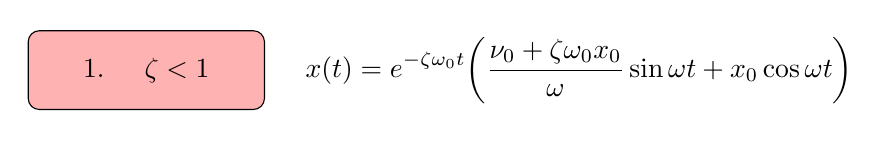
\begin{tikzpicture}
    \node (start) [start] {1. \quad $\zeta < 1$};
    \node (text) [rectangle, right of = start, xshift = 4.5cm] {$\displaystyle x(t) = e^{- \zeta \omega_0 t} \bigg( \frac{\nu_0 + \zeta \omega_0 x_0}{\omega} \sin \omega t + x_0 \cos \omega t \bigg) $};
\end{tikzpicture}

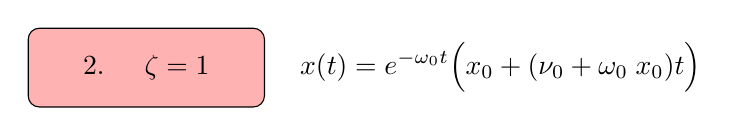
\begin{tikzpicture}
    \node (start) [start] {2. \quad $\zeta = 1$};
    \node (text) [rectangle, right of = start, xshift = 3.5cm] {$\displaystyle x(t) = e^{-\omega_0 t} \Big( x_0 + (\nu_0 + \omega_0 \; x_0) t \Big) $};
\end{tikzpicture}

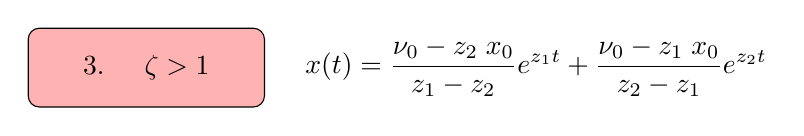
\begin{tikzpicture}
    \node (start) [start] {3. \quad $\zeta > 1$};
    \node (text) [rectangle, right of = start, xshift = 3.95cm] {$\displaystyle x(t) = \frac{\nu_0 - z_2 \; x_0}{z_1 - z_2} e^{z_1 t} + \frac{\nu_0 - z_1 \; x_0}{z_2 - z_1} e^{z_2 t} $};
\end{tikzpicture}







%% Amortissement d'une perturbation initiale
\begin{center}
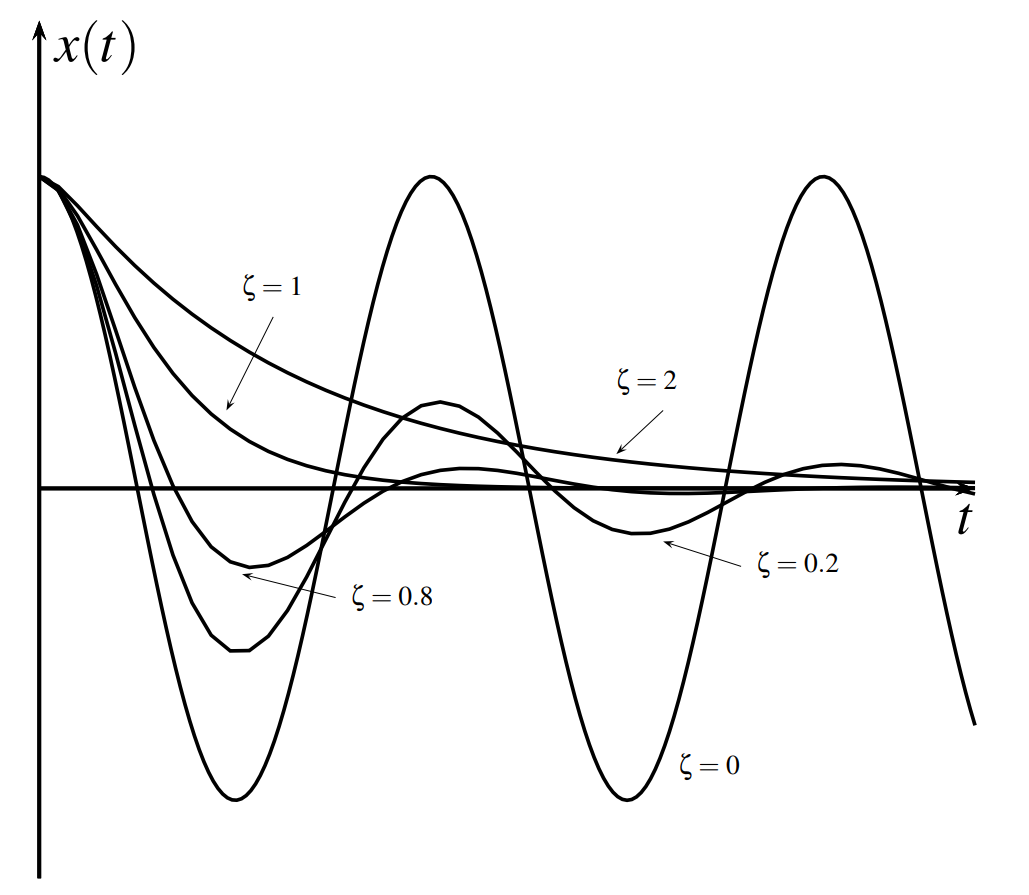
\includegraphics[width=0.5\textwidth]{images/Amortissement.PNG}
\end{center}

\item Lorsque $ \zeta = 0 $, il n'y a pas d'amortissement. Si $ \zeta < 1 $, La solution est oscillatoire et l'amortissement est dit "sous-critique". Dans le cas où $ \zeta = 1 $, l'amortissement est dit critique, alors que lorsque $ \zeta > 1 $, l'amortissement est "sur-critique".





%% Frottement sec
\item Dans le cas d'un frottement sec, la force de liaison entre le mobile et le plan possède une composante verticale $\displaystyle N \; \textbf{e}_y $ et une composante horizontale $\displaystyle T \; \textbf{e}_x $ où $ T $ vaut : 
\[ T = - \mu \; N \text{ sign} (\dot{x}) \]

\begin{center}
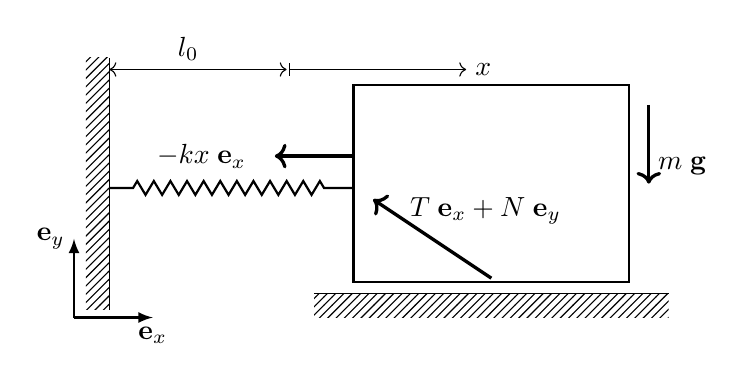
\begin{tikzpicture}[every node/.style={draw,outer sep=0pt,thick}]
\tikzstyle{spring}=[thick,decorate,decoration={zigzag,pre length=0.3cm,post length=0.3cm,segment length=6}]

\tikzstyle{ground}=[fill,pattern=north east lines,draw=none,minimum width=0.75cm,minimum height=0.3cm]



\begin{scope}[xshift=7cm]
\node (M) [minimum width=3.5cm, minimum height=2.5cm] {};

\node (ground) [ground,anchor=north,yshift=-0.15cm,minimum width=4.5cm] at (M.south) {};
\draw (ground.north east) -- (ground.north west);

\node (wall) [ground, rotate=-90, minimum width=3.2cm,yshift=-5cm] {};
\draw (wall.north east) -- (wall.north west);

\draw [spring] (wall.70) -- ($(M.north west)!(wall.70)!(M.south west)$) node[pos=.5,left, draw=none, yshift = 0.4cm, xshift=0.3cm]{$ -k x \; \textbf{e}_x $};

\draw [-latex, thick, xshift = -5.3cm, yshift = -1.7cm] (0,0) -- +(1cm,0) node[anchor=north, draw = none]{$ \textbf{e}_x $};
\draw [-latex, thick, xshift = -5.3cm, yshift = -1.7cm] (0,0) -- +(0,1cm) node[anchor=east, draw = none]{$ \textbf{e}_y $};

\draw [<->, xshift = -4.85cm, yshift = 1.45cm] (0,0) -- (2.25cm,0) node[anchor=south, draw=none, xshift=-1.25cm]{$ l_0 $};
\draw [|->, xshift = -2.57cm, yshift = 1.45cm] (0,0) -- (2.25cm,0) node[anchor=west, draw=none]{$ x $};

\draw [->, very thick, xshift = 2cm] (0,1cm) -- (0,0) node[anchor=south west, draw=none]{$ m\; \textbf{g} $};
\draw [->, very thick, yshift = -1.2cm] (0,0) -- (-1.5cm, 1cm) node[anchor=west, draw=none, xshift=0.35cm, yshift=-0.15cm]{$ T \; \textbf{e}_x + N \; \textbf{e}_y $};
\draw [->, very thick, xshift=-1.75cm, yshift=0.35cm] (0,0) -- (-1cm,0);

\end{scope}
\end{tikzpicture}
\end{center}

La loi de Newton s'écrit : 
\[ m \; \ddot{x} \; \textbf{e}_x = (-k \; x + T) \; \textbf{e}_x + (N - m \; g) \; \textbf{e}_y \]
de sorte que (en posant $ \omega_0 = \sqrt{k/m} $) : 
\[ \begin{cases}
\ddot{x} + \omega_0^2 \; x = - \mu \; g \quad & \text{ si } \dot{x} > 0 \\
\ddot{x} + \omega_0^2 \; x = \mu \; g & \text{ si } \dot{x} < 0
\end{cases} \]

Si $ x > 0 $ ($ \dot{x}_0 = 0 $), on a : 
\[ x(t) = \frac{\mu \; g}{\omega_0^2} + \bigg( x_0 - \frac{\mu \; g}{\omega_0^2} \bigg) \cos \omega_0 t \qquad \text{ pour } t \in \; \Big] 0, \frac{\pi}{\omega_0} \Big[ \]
Ensuite, on aura $ x < 0 $ ($ \dot{x}_0 = 0 $) et donc : 
\[ x(t) = - \frac{\mu \; g}{\omega_0^2} + \bigg( x_0 - \frac{3 \mu \; g}{\omega_0^2} \bigg) \cos \omega_0 t \qquad \text{ pour } t \in \; \Big] \frac{\pi}{\omega_0}, \frac{2 \pi}{\omega_0} \Big[ \]
Après chaque intervalle de temps $\displaystyle \frac{\pi}{\omega_0} $, l'amplitude de l'oscillation est réduite, si bien que après un moment, la force de friction devient supérieure à la force de rappel du ressort.

\begin{center}
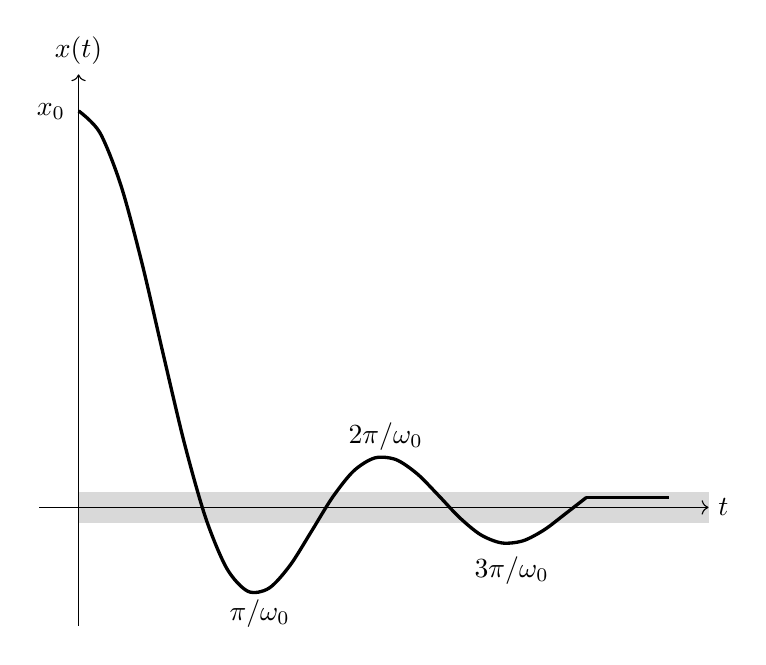
\begin{tikzpicture}
    \draw[->] (-0.5,0) -- (8,0) node[right] {$ t $};
    \draw[->] (0,-1.5) -- (0,5.5) node[above] {$ x(t) $};

    \draw[color=black, smooth, very thick, domain=0.001:6.45]   plot (\x,{ 2.5 * sin(\x r * 2) / \x }) node[draw=none, xshift=-6.8cm, yshift=4.9cm]{$ x_0 $};
    \draw[-, color=black, very thick] (6.45,0.1269) -- (7.5,0.1269);

\begin{scope}[on background layer]
    \node [rectangle, draw=none,minimum width=8cm, xshift = 4cm, minimum height=0.4cm, fill=black!15]{};
\end{scope}

    \node [xshift=2.3cm, yshift=-1.35cm] {$ \pi/\omega_0 $};
    \node [xshift=3.9cm, yshift=0.9cm] {$ 2\pi/\omega_0 $};
    \node [xshift=5.5cm, yshift=-0.8cm] {$ 3\pi/\omega_0 $};
\end{tikzpicture}
\end{center}





%% Oscillateurs harmoniques couplés
\item Oscillateurs harmoniques couplés : \\
La réponse libre d'oscillateurs harmoniques couplés consiste en une oscillation composite, superposition de plusieurs oscillations périodiques dont les fréquences sont les \emph{fréquences propres} du système. La forme particulière des oscillations harmoniques correspondant à chacune des fréquences propres est appelée \emph{mode de vibration}.

\begin{center}
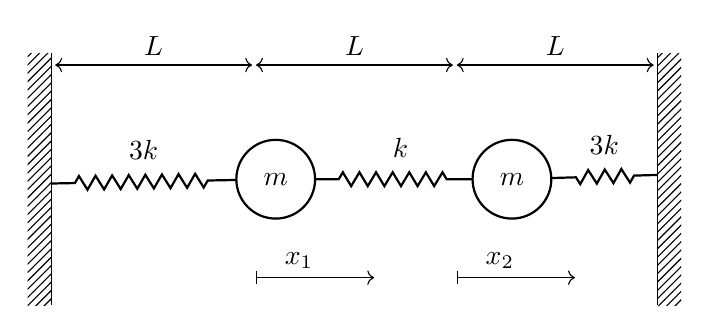
\begin{tikzpicture}[every node/.style={draw,outer sep=0pt,thick}]
\tikzstyle{spring}=[thick,decorate,decoration={zigzag,pre length=0.3cm,post length=0.3cm,segment length=6}]

\tikzstyle{ground}=[fill,pattern=north east lines,draw=none,minimum width=0.75cm,minimum height=0.3cm]


\begin{scope}[xshift=7cm]
\node (M) [circle, thick, minimum size=1cm] {$ m $};
\node (M2) [circle, thick, minimum size=1cm, xshift=3cm] {$ m $};

\node (wall) [ground, rotate=-90, minimum width=3.2cm,yshift=-3cm] {};
\draw (wall.north east) -- (wall.north west);

\node (wall2) [ground, rotate=90, minimum width=3.2cm,yshift=-5cm] {};
\draw (wall2.north east) -- (wall2.north west);

\draw [spring] (wall.70) -- (M) node[pos=.5,left, draw=none, yshift = 0.4cm, xshift=0.3cm]{$ 3 k $};
\draw [spring] (M) -- (M2) node[pos=.5,left, draw=none, yshift = 0.4cm, xshift=0.3cm]{$ k $};
\draw [spring] (wall2.70) -- (M2) node[pos=.5,left, draw=none, yshift = 0.4cm, xshift=0.3cm]{$ 3 k $};

\draw [<->, xshift = -2.8cm, yshift = 1.45cm] (0,0) -- (2.5cm,0) node[anchor=south, draw=none, xshift=-1.25cm]{$ L $};
\draw [<->, xshift = -0.25cm, yshift = 1.45cm] (0,0) -- (2.5cm,0) node[anchor=south, draw=none, xshift=-1.25cm]{$ L $};
\draw [<->, xshift = 2.3cm, yshift = 1.45cm] (0,0) -- (2.5cm,0) node[anchor=south, draw=none, xshift=-1.25cm]{$ L $};

\draw [|->, xshift = -0.25cm, yshift = -1.25cm] (0,0) -- (1.5cm,0) node[anchor=south west, draw=none, xshift=-1.25cm]{$ x_1 $};
\draw [|->, xshift = 2.3cm, yshift = -1.25cm] (0,0) -- (1.5cm,0) node[anchor=south west, draw=none, xshift=-1.25cm]{$ x_2 $};

\end{scope}
\end{tikzpicture}
\end{center}

Si on place les axes à la longueur naturelle des ressorts, les équations du mouvement s'écrivent : 
\[ \begin{aligned} m \ddot{x}_1 + 3 k x_1 - k (x_2 - x_1) &= 0 \\ m \ddot{x}_2 + 3 k x_2 - k (x_1 - x_2) &= 0 \end{aligned} \]
On découple ces équations en posant : 
\[ \begin{aligned} X_1 &= x_1 + x_2 \\ X_2 &= x_1 - x_2 \end{aligned} \qquad \qquad \begin{aligned} 2 x_1 &= X_1 + X_2 \\ 2 x_2 &= X_1 - X_2 \end{aligned} \]
D'un point de vue physique, $ X_1 $ décrit le déplacement du centre d'inertie du système. \\
On obtient alors : 
\[ \begin{aligned} m \ddot{X}_1 + 3 k X_1 &= 0 \\ m \ddot{X}_2 + 5 k X_2 &= 0 \end{aligned} \qquad \implies \qquad
\begin{aligned} X_1 &= C_1 \cos (\sqrt{3} \; \omega_0 t + \varphi_1) \\ X_2 &= C_2 \cos (\sqrt{5} \; \omega_0 t + \varphi_2) \end{aligned} \]
où $ \omega_0^2 = k/m $. Les fréquences propres du systèmes sont donc $ \omega_I = \sqrt{3} \; \omega_0 $ et $ \omega_{II} = \sqrt{5} \; \omega_0 $.
\begin{center} \begin{tabular}{lll}
Si $ x_1 = x_2 $, & les 2 points matériels oscillent en phase & (fréquence $ = \omega_I $) \cr
Si $ x_1 = - x_2 $, & les 2 points matériels oscillent en opposition de phase & (fréquence $ = \omega_{II} $)
\end{tabular} \end{center}





%% Oscillateurs harmoniques couplés - forçage périodique
\item Dans le cas envisagé, si on applique une force \textbf{F} au premier point matériel du système telle que $ F = m L \Omega^2 \cos \omega t $, on a : 
\[ \begin{aligned} m \ddot{x}_1 + 3 k x_1 - k (x_2 - x_1) &= m L \Omega^2 \cos \omega t \\ m \ddot{x}_2 + 3 k x_2 - k (x_1 - x_2) &= 0 \end{aligned} \qquad \implies \qquad 
\begin{aligned} m \ddot{X}_1 + 3 k X_1 &= m L \Omega^2 \cos \omega t \\ m \ddot{X}_2 + 5 k X_2 &= m L \Omega^2 \cos \omega t \end{aligned} \]
On peut donc étudier séparément la réponse de chacun des modes propres soumis à une force excitatrice. On dit de cette force s'appliquant à un mode particulier qu'elle est la \emph{projection de la force appliquée dans la base des modes propres}. \\
Et si $ x_1 = x_2 = 0 \; ; \; \dot{x}_1 = \dot{x}_2 = 0 $, on a : 
\[ X_1 = \frac{L \Omega^2}{\omega_I^2 - \omega^2} (\cos \omega t - \cos \omega_I t) \qquad \qquad X_2 = \frac{L \Omega^2}{\omega_{II}^2 - \omega^2} (\cos \omega t - \cos \omega_{II} t) \]
Si $ \omega = \omega_I $ ou si $ \omega = \omega_{II} $, alors il y a résonance et la solution ci-dessus n'est plus correcte. Par exemple, si $ \omega = \omega_I $, on a : 
\[ X_1 = \frac{L \Omega^2}{2 \omega_I} t \sin \omega_I t \]





%% Note sur les modes propres
\item Note sur les modes propres : \\
Un mode normal ou mode propre d'oscillation est une forme de mouvement dans laquelle toutes les parties du système se déplacent sinusoïdalement avec la même fréquence naturelle de vibration associée au mode. \\
Le nombre de modes normaux est égal à celui des degrés de liberté du système.

Le mouvement général d'un système est la superposition de ses modes normaux. Les modes sont normaux dans le sens qu'ils se déplacent indépendamment les uns des autres, une excitation d'un des modes ne cause jamais le mouvement d'un autre mode. En termes mathématiques, les modes sont orthogonaux.






\end{itemize}




















\section{Applications : Mouvement de base du point matériel}










\begin{itemize}





%% Chute dans le vide
\item Lors d'une chute dans le vide, la seule force agissant sur un corps de masse m est $ m \; \textbf{g} $. L'équation \emph{différentielle} vectorielle du mouvement est donc : $ m \; \ddot{\textbf{s}} = m \; \textbf{g} $. Son équation du mouvement est donc : 
\[ \textbf{s}(t) = \frac{1}{2} \textbf{g} \; t^2 + \textbf{v}_0 \; t + \textbf{s}_0 \]





%% Chute en milieu résistif
\item Si la résistance de l'air créé une force $ \textbf{F} = - k \; \dot{\textbf{s}} $, l'EDVM (équation différentielle vectorielle du mouvement) s'écrit : 
\[ m \; \ddot{\textbf{s}} = m \; \textbf{g} - k \; \dot{\textbf{s}} \]
Son EM (équation de mouvement) s'écrit quant à elle : 
\begin{align*}
\textbf{s}(t) &= \textbf{C}_1 + \textbf{C}_2 \; e^{- k t / m} + \frac{m \; \textbf{g}}{k} t \\
&= h \; \textbf{E}_z + \frac{m^2 \; \textbf{g}}{k^2} \Big( e^{- k t / m} - 1 \Big) + \frac{m \; \textbf{g}}{k} t \\
z(t) &= h + \frac{m^2 \; g}{k^2} \Big( 1 - e^{- k t / m} \Big) - \frac{m \; g}{k} t
\end{align*}
La vitesse du corps augmente et tend progressivement vers la vitesse limite de chute : $\displaystyle v_L = \frac{m \; g}{k} $.





%% Projectile
\item La seule force agissant sur le projectile est la pesanteur. On a donc : $\displaystyle m \; \ddot{\textbf{s}} = m \; \textbf{g} $.

\begin{center}
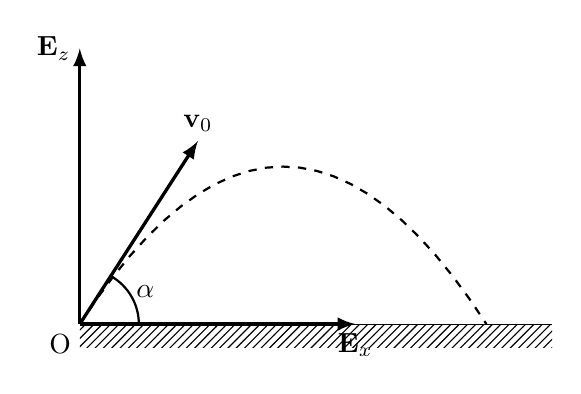
\begin{tikzpicture}[every node/.style={draw,outer sep=0pt,thick}]

\tikzstyle{ground}=[fill,pattern=north east lines,draw=none,minimum width=0.75cm,minimum height=0.3cm]



\begin{scope}[xshift=7cm]

\node (ground) [ground,anchor=north,xshift=3cm,minimum width=6cm]{};
\draw (ground.north east) -- (ground.north west);

\draw [-latex, very thick, xshift = 0cm, yshift = 0cm] (0,0) -- +(3.5cm,0) node[anchor=north, draw = none]{$ \textbf{E}_x $};
\draw [-latex, very thick, xshift = 0cm, yshift = 0cm] (0,0) -- +(0,3.5cm) node[anchor=east, draw = none]{$ \textbf{E}_z $};

\draw[color=black, dashed, thick, domain=0.001:5.164]   plot (\x,{- 0.3 * (\x - 2.582)^2 + 2}){};

\draw [-latex, very thick] (0,0) -- +(1.5,2.3238) node[anchor=south, draw=none]{$ \textbf{v}_0 $};
\draw [-, thick] (0.75,0) arc (0:60:.7cm) node[anchor=north west, draw=none, xshift=0.2cm]{$ \alpha $};

\node (origin) [xshift= -0.25cm, yshift= -0.25cm, draw=none]{O};

\end{scope}
\end{tikzpicture}
\end{center}

En intégrant, on obtient : 
\[ \dot{\textbf{s}} = \textbf{g} \; t + v_0 (\cos \alpha \; \textbf{E}_x + \sin \alpha \; \textbf{E}_z) \qquad \qquad \qquad \textbf{s}(t) = \frac{1}{2}\textbf{g}t^2 + v_0 \; t (\cos \alpha \; \textbf{E}_x + \sin \alpha \; \textbf{E}_z) \]





%% Mouvement dans un champ électromagnétique
\item Une particule de masse m, charge q dans un champ électromagnétique est soumise à la force : $\displaystyle \textbf{F} = q (\textbf{E} + \textbf{v} \wedge \textbf{B}) $ qui se réécrit sous la forme : $\displaystyle m \; \ddot{\textbf{s}} = q (\textbf{E} + \dot{\textbf{s}} \wedge \textbf{B}) $. \\
On pose : 
\[ \textbf{e} = \frac{q}{m} \textbf{E} \; \; ; \; \; \omega_c = - \frac{q \; B}{m} \; \; ; \; \; \textbf{b} = \frac{\textbf{B}}{\| \textbf{B} \|} \]
Ce qui nous donne : $\displaystyle \ddot{\textbf{s}} = \textbf{e} + \omega_c \; \textbf{b} \wedge \dot{\textbf{s}} $.





%% B = 0
\item Si $ \textbf{B} = \textbf{0} $, alors $ \ddot{\textbf{s}} = \textbf{e} $ et donc : $\displaystyle \textbf{s} = \frac{1}{2} \textbf{e} \; t^2 + \textbf{v}_0 \; t + \textbf{s}_0 $.





%% E = 0
\item Si $ \textbf{E} = \textbf{0} $, alors $ \ddot{\textbf{s}} = \omega_c \; \textbf{b} \wedge \dot{\textbf{s}} $.
\begin{center}
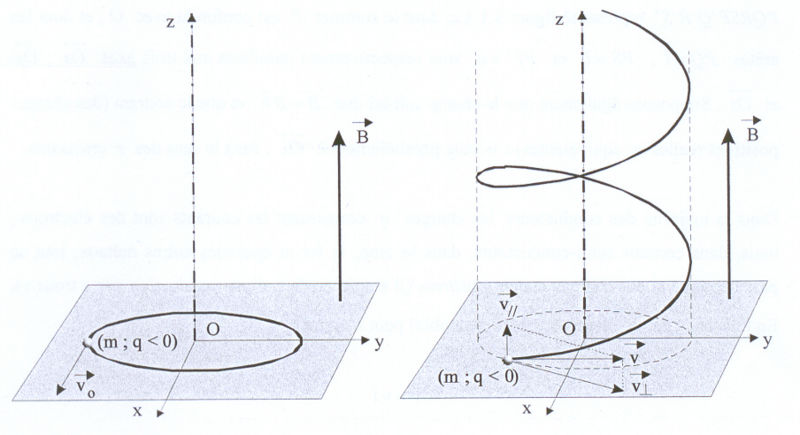
\includegraphics{images/Trajectoire.jpg}
\end{center}

\begin{enumerate}
\item Vitesse initiale perpendiculaire au champ : 
\[ \textbf{F} = q \; \textbf{v} \wedge \textbf{B} = m \; \textbf{a} \qquad \qquad \text{ où } a = a_c = \frac{v^2}{r} \qquad \qquad \textbf{v} \perp \textbf{B} \implies F = q \; v \; B \]
\[ q \; v \; B = m \frac{v^2}{r} \implies r = \frac{m \; v}{q \; B} = \frac{\fbox{m v}}{\fbox{q B}} \]
$\displaystyle \longrightarrow \fbox{m v} $ est la quantité de mouvement \\
$\displaystyle \longrightarrow \fbox{q B} $ est l'interaction électrostatique

En physique des particules chargées, $\displaystyle r = \frac{m \; v}{q \; B} $ est appelé rayon cyclotronique et $\displaystyle \omega_c = \frac{v}{r} = \frac{q \; B}{m} $ porte le nom de fréquence cyclotronique (elle est souvent notée $ \omega = \frac{|q| \; B}{m} $).
\item Vitesse initiale perpendiculaire au champ : \\
Si on note $ \textbf{v}_{\parallel} $ la vitesse parallèle à $ \textbf{B} $ et $ \textbf{v}_{\perp} $ la vitesse perpendiculaire à $ \textbf{B} $, on a : $\displaystyle r = \frac{m \; v_\perp}{q \; B} \implies v_\perp = \frac{q \; B \; r}{m} $. \\
Le pas de l'hélice (le mouvement en 3d est hélicoïdal) vaut : $\displaystyle z = v_\parallel \; T $ avec T la période qui vaut : $\displaystyle T = \frac{2 \pi \; r}{v_\perp} = \frac{2 \pi \; m}{q \; B} $.
\[ z = 2 \pi \frac{m \; v_\parallel}{q \; B} = 2 \pi \frac{\fbox{m $ v_\parallel $}}{\fbox{q B}} \]
\end{enumerate}





%% Expression vectorielle de la trajectoire d'une particule chargée dans un champ magnétique
\item Expression vectorielle de la trajectoire d'une particule chargée dans un champ magnétique : 
\[ \textbf{s}(t) = v_\parallel \; t \; \textbf{E}_z + r\;  \big( \cos \theta \; \textbf{E}_x + \sin \theta \; \textbf{E}_y \big) \]
où $ \theta (t) $ vaut $ 2 \pi $ en $ t = T = 2 \pi / m q B \implies \theta = t \; m \; q \; B $.





%% Mouvement des systèmes à masse variable
\item Dans un système à masse variable (SMV), l'EDVM s'écrit : 
\[ m(t) \; \ddot{\textbf{s}} = \textbf{G} + \textbf{P} \]
où \textbf{s} est le vecteur position du centre d'inertie (CI) du SMV, \textbf{G} est la résultante des forces qui agissent sur le SMV et \textbf{P} est la poussée avec $\displaystyle \textbf{P} = \frac{d m}{d t} \textbf{w} $. \\
\[ \frac{d m}{d t} \; \begin{cases}
> 0 \; \text{ si absorption (m augmente) } \\
< 0 \; \text{ si éjection (m baisse) }
\end{cases} \qquad \text{ \danger Attention aux erreurs de signe ! } \]
\textbf{w} est la vitesse de l'objet absorbé/éjecté par rapport au SMV (vitesse relative).





%% Relation différentielle utile
\item Relation différentielle utile lorsqu'on a une force divisible par $ \dot{z}^2 $ (ex : si $ \textbf{F} = - k \; \dot{\textbf{z}}^2 $) : 
\[ \frac{d^2 z}{d t^2} = \frac{1}{2} \frac{d}{d z} (\dot{z}^2) \]





\end{itemize}




















\section{Applications : Mouvements guidés}










\begin{itemize}





%% Pendule simple
\item L'équation de Newton d'un pendule simple s'écrit : $\displaystyle m \; \ddot{\textbf{s}} = m \; \textbf{g} + \textbf{R} $ avec $ \textbf{R} = \textbf{R}_\nu + \textbf{B}_\beta $.

\begin{center}
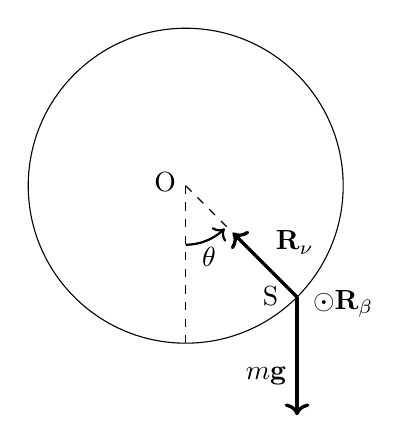
\begin{tikzpicture}
\draw [black] (0,0) circle [radius=2];
\draw [-, dashed] (0,0) -- node[anchor=south east, yshift=0.8cm]{O} (0,-2);
\draw [-, dashed] (0,0) -- node[anchor=north west, yshift=-0.45cm, xshift=0.15cm]{S} (1.414,-1.414);
\draw [->, very thick] (1.414,-1.414) -- node[anchor=north east]{$ m \textbf{g} $} (1.414,-2.914);
\draw [->, thick] (0,-0.75) arc (-90:-45:.7cm) node[anchor=north, draw=none, xshift = -0.2cm, yshift=-0.1cm]{$ \theta $};
\draw [->, very thick] (1.414,-1.414) -- node[anchor=south west]{$ \textbf{R}_\nu $} (0.6,-0.6);
\node [draw=none] at (2,-1.5) {$ \odot \textbf{R}_\beta $};
\end{tikzpicture}
\end{center}

Pour se débarrasser du terme $ \textbf{R} $, on multiplie l'équation par $ \dot{\textbf{s}} $ : $\displaystyle \ddot{\textbf{s}} \cdot \dot{\textbf{s}} = \textbf{g} \cdot \dot{\textbf{s}} $. \\
On en tire l'\emph{intégrale première} de conservation de l'énergie : $\displaystyle \frac{1}{2} \| \dot{\textbf{s}} \|^2 = \textbf{g} \cdot\textbf{s} + c $ où $ c $ est une constante. On écrit donc : $\displaystyle \frac{1}{2} \| \dot{\textbf{s}} \|^2 - \textbf{g} \cdot\textbf{s} = c = e $ (on note e l'énergie du système par unité de masse). \\
On pose $\displaystyle z = 0 \; ; \; r = a \; ; \; \omega^2 = \frac{g}{a} $ et puisque la position ne varie qu'en fonction de $ \theta $, l'équation devient : 
\[ \underbrace{\frac{1}{2 \omega^2} \dot{\theta}^2}_{E_{cin}} \underbrace{- \cos \theta}_{E_{pot}} = \underbrace{e}_{E_{tot}}  \quad \implies \quad \underbrace{\frac{1}{2 \omega^2} \dot{\theta}^2}_{> 0} = \underbrace{e + \cos \theta}_{> 0} \]
Étant donné que $\displaystyle e + \cos \theta > 0 $, nous avons une nouvelle équation : 
\[ e > \underbrace{- \cos \theta}_{V(\theta)} \]

\begin{center}
\begin{tikzpicture}
    \draw[->] (-5,0) -- (9,0) node[right] {$ \theta $};
    \draw[->] (0,-3.5) -- (0,3.5) node[right] {$ V(\theta) $};

    \draw[color=black, smooth, very thick, domain=-4:8]   plot (\x,{ - 2.5 * cos(\x r) });

    \draw[-, dashed] (-5,2.5) -- (7,2.5) node[right] {$ e = 1 $};
    \draw[-, dashed] (-5,1.5) -- (7,1.5) node[right] {$ -1 < e < 1 $};
    \draw[-, dashed] (-5,-2.5) -- (7,-2.5) node[right] {$ e = -1 $};
\end{tikzpicture}
\end{center}

Le mouvement n'est possible que si $ e \geq -1 $. Si $ e = -1 + \epsilon $, alors $ \theta \ll 1 $.
L'équation $\displaystyle \frac{1}{2 \omega^2} \dot{\theta}^2 - \cos \theta = e $ peut dés lors être réécrite sous la forme : $\displaystyle \frac{1}{2 \omega^2} \dot{\theta}^2 - \Big( 1 - \frac{\theta^2}{2} \Big) = -1 + \epsilon $. On la dérive par $ t $ et on obtient : $\displaystyle \ddot{\theta} + \omega^2 \theta = 0 \quad \implies \quad \theta(t) = A \cos \omega t + B \sin \omega t $. Ou alternativement, $\displaystyle \theta = C_1 \cos (\omega t + \Phi_0) $.





%% Pendule rotatif
\item Pendule rotatif : 
\NoIndent{
\begin{center} \begin{tabular}{M{5cm}M{6cm}M{5cm}}
\begin{center}
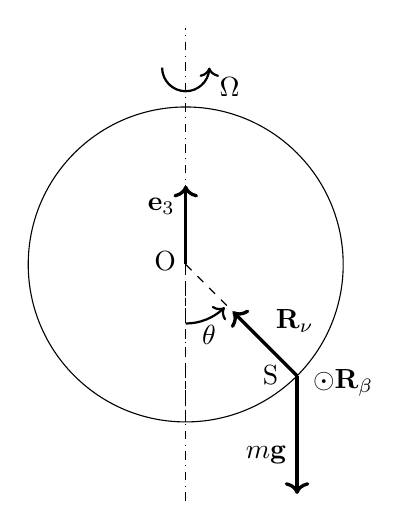
\begin{tikzpicture}
\draw [-, dash dot] (0,-3) -- (0,3);
\draw [black] (0,0) circle [radius=2];
\draw [-, dashed] (0,0) -- node[anchor=south east, yshift=0.8cm]{O} (0,-2);
\draw [-, dashed] (0,0) -- node[anchor=north west, yshift=-0.45cm, xshift=0.15cm]{S} (1.414,-1.414);
\draw [->, very thick] (1.414,-1.414) -- node[anchor=north east]{$ m \textbf{g} $} (1.414,-2.914);
\draw [->, thick] (0,-0.75) arc (-90:-45:.7cm) node[anchor=north, draw=none, xshift = -0.2cm, yshift=-0.1cm]{$ \theta $};
\draw [->, very thick] (1.414,-1.414) -- node[anchor=south west]{$ \textbf{R}_\nu $} (0.6,-0.6);
\node [draw=none] at (2,-1.5) {$ \odot \textbf{R}_\beta $};
\draw [->, very thick] (0,0) -- node[anchor=south east]{$ \textbf{e}_3 $} (0,1);
\draw [->, thick] (-0.3,2.5) arc (-180:0:.3cm) node[anchor=north west, draw=none, xshift=0cm, yshift=0cm]{$ \Omega $};
\end{tikzpicture}
\end{center}
&
\begin{center}
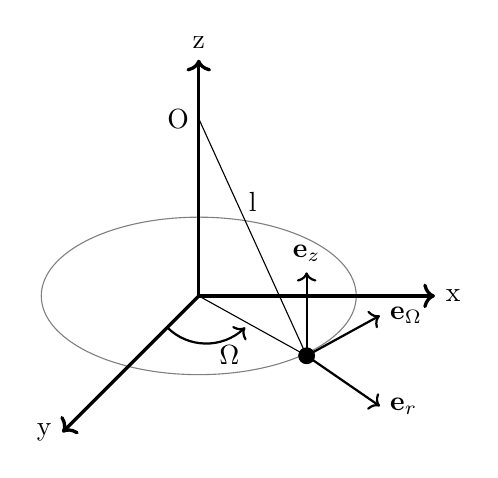
\begin{tikzpicture}
\draw (0,0) [draw=gray] ellipse (2cm and 1cm);
\draw [->, very thick] (0,0) -- (3,0) node[anchor=west]{x};
\draw [->, very thick] (0,0) -- (0,3) node[anchor=south]{z};
\draw [->, very thick] (0,0) -- (-1.732,-1.732) node[anchor= east]{y};
\draw [->, thick] (-0.4,-0.4) arc (-135:-45:.7cm) node[anchor=north, draw=none, xshift = -0.2cm, yshift=-0.1cm]{$ \Omega $};
\draw [-] (0,0) -- (1.37,-0.76);
\draw [black, fill=black] (1.37,-0.76) circle [radius=0.1];

\draw [->, thick] (1.37,-0.76) -- (2.3,-1.4) node[anchor=west]{$ \textbf{e}_r $};
\draw [->, thick] (1.37,-0.76) -- (1.37,0.3) node[anchor=south]{$ \textbf{e}_z $};
\draw [->, thick] (1.37,-0.76) -- (2.3,-0.25) node[anchor=west]{$ \textbf{e}_\Omega $};
\draw [-] (0,2.25) node[anchor=east]{O} -- node[anchor=south, yshift=0.2cm]{l} (1.37,-0.76);
\end{tikzpicture}
\end{center}
&
\begin{center}
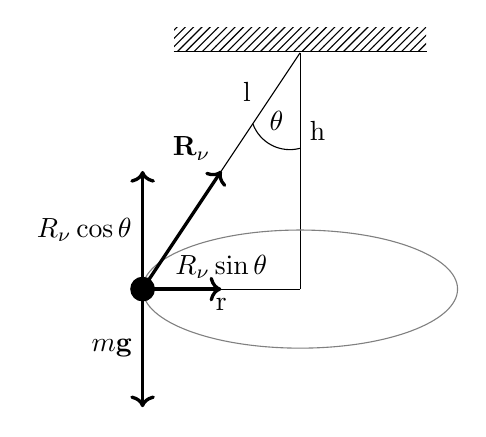
\begin{tikzpicture}
\tikzstyle{ground}=[fill,pattern=north east lines,draw=none,minimum width=0.75cm,minimum height=0.3cm]
\node (wall) [ground, rotate=-180, minimum width=3.2cm, yshift=-3.17cm] {};
\draw (wall.north east) -- node[anchor=west, yshift=-1cm]{h} (wall.north west);

\draw [-] (0,3) -- (0,0);
\draw (0,0) [draw=gray] ellipse (2cm and 0.75cm);
\draw [black, fill=black] (-2,0) circle [radius=0.15];
\draw [-] (-2,0) -- node[anchor=east, xshift=0.5cm, yshift=1cm]{l} (0,3);
\draw [-, xshift = -0.6cm, yshift = 0.6cm] (0,1.5) arc (200:285:.5cm) node[anchor=south, draw=none, xshift = -0.3cm, yshift=0.1cm]{$ \theta $};
\draw [-] (0,0) -- node[anchor=north]{r} (-2,0);
\draw [->, very thick] (-2,0) -- node[anchor=east]{$ m \textbf{g} $} (-2,-1.5);
\draw [->, very thick] (-2,0) -- (-1,1.5) node[anchor=south east]{$ \textbf{R}_\nu $};
\draw [->, very thick] (-2,0) -- node[anchor=east]{$ R_\nu \cos \theta $} (-2,1.5);
\draw [->, very thick] (-2,0) -- node[anchor=south, xshift=0.5cm]{$ R_\nu \sin \theta $} (-1,0);

\end{tikzpicture}
\end{center}
\end{tabular} \end{center}}

Un pendule rotatif qui tourne à vitesse constante $ \Omega $ autour de l'axe $ \textbf{e}_3 $ possède un vecteur de Poisson : $ \boldsymbol{\Omega} = \Omega \; \textbf{e}_3 $. \\
L'équation de Newton en axes relatifs s'écrit : 
\[ \underbrace{m \frac{\delta^2 \textbf{s}}{\delta t^2}}_{relative} + \underbrace{2 m \; \boldsymbol{\Omega} \wedge \frac{\delta \textbf{s}}{\delta t}}_{coriolis} + \underbrace{m \; \boldsymbol{\Omega} \wedge (\boldsymbol{\Omega \wedge \textbf{s}})}_{entrainement} = m \; \textbf{g} + \textbf{R} \]
En multipliant scalairement par la vitesse relative  et en développant le produit vectoriel $ \big( \textbf{a} \wedge (\textbf{b} \wedge \textbf{c}) = (\textbf{a} \cdot \textbf{c}) \textbf{b} - (\textbf{a} \cdot \textbf{b}) \textbf{c} \big) $, on arrive à une équation immédiatement intégrable : $\displaystyle \frac{\delta^2 \textbf{s}}{\delta t^2} \cdot \frac{\delta \textbf{s}}{\delta t} + (\boldsymbol{\Omega} \cdot \textbf{s}) \Big( \boldsymbol{\Omega} \cdot \frac{\delta \textbf{s}}{\delta t} \Big) - \Omega^2 \textbf{s} \cdot \frac{\delta \textbf{s}}{\delta t} = \textbf{g} \cdot \frac{\delta \textbf{s}}{\delta t} $.
On en tire : 
\[ \frac{1}{2} \Big\| \frac{\delta \textbf{s}}{\delta t} \Big\|^2 + \frac{1}{2} (\boldsymbol{\Omega} \cdot \textbf{s})^2 - \frac{1}{2} \Omega^2 \| \textbf{s} \|^2 = \textbf{g} \cdot \textbf{s} + c \]
On peut écrire : $\displaystyle \textbf{s} = l \; \textbf{e}_r \; ; \; \frac{\delta \textbf{s}}{\delta t} = l \dot{\theta} \; \textbf{e}_\theta $ et on pose : $\displaystyle n = \frac{\Omega}{\omega} \; ; \; \omega = \sqrt{\frac{g}{l}} $. Ce qui nous permet de réécrire l'équation précédente : 
\[ \mathring{\theta}^2 \underbrace{- (n^2 \sin^2 \theta + 2 \cos \theta)}_{V(\theta)} = 2 \; c \]

\begin{center}
    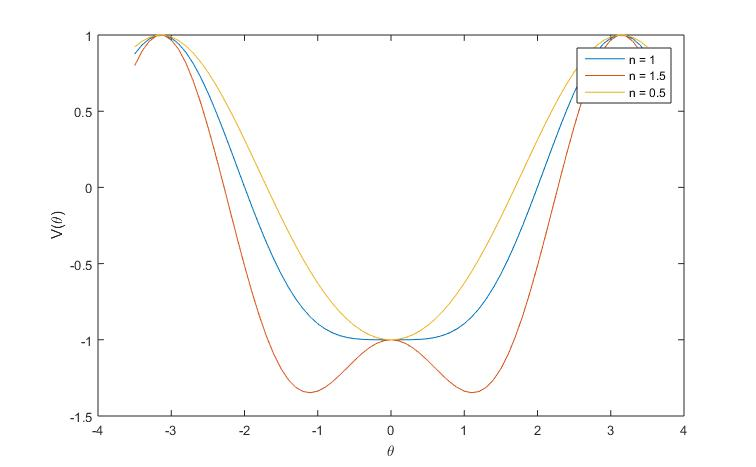
\includegraphics[width=0.9\textwidth]{images/pendule_rotatif.jpg}
\end{center}





%% Analyse des position d'équilibre du pendule rotatif
\item Analyse des position d'équilibre du pendule rotatif $ \Big( \ringring{\theta} = \sin \theta (n^2 \cos \theta - 1) \Big) $ : 
\begin{itemize}
\item Positions d'équilibre : $ \theta = \theta_{\text{eq}} \implies \mathring{\theta} = 0 \; ; \; \ringring{\theta} = 0 $.
    \begin{itemize}
    \item $ \sin \theta_{\text{eq}} = 0 \implies \theta_{\text{eq}} = 0, \; \pm \pi $
    \item $ n^2 \cos \theta_{\text{eq}} - 1 = 0 \implies \theta_{\text{eq}} = \pm \arccos \frac{1}{n^2} $ si $ n^2 \geq 1 $
    \end{itemize}
\item Méthode des perturbations infinitésimales : \\
Si on note $ \epsilon $ la perturbation, on a l'équation : $ \ringring{\epsilon} + (1 - n^2) = 0 $
    \begin{itemize}
        \item $ n^2 < 1 $, \quad $ \epsilon(\tau) = A \sin \sqrt{1 - n^2} \; \tau + B \cos \sqrt{1 - n^2} \; \tau \longrightarrow $ Marginalement stable
        \item $ n^2 > 1 $, \quad $ \epsilon(\tau) = A \text{ sh } \sqrt{n^2 - 1} \; \tau + B \text{ ch } \sqrt{n^2 - 1} \; \tau \longrightarrow $ Instable
        \item $ n^2 = 1 $, \quad $ \ringring{\epsilon} = 0 \implies \epsilon(\tau) = A + B \tau \longrightarrow $ Faiblement instable
    \end{itemize}
\item Méthode des petites perturbations : \\
On a : $\displaystyle \ringring{\epsilon} \approx - \frac{\epsilon^3}{2} \implies \ringring{\epsilon} + \frac{\epsilon^3}{2} = 0 \implies \frac{1}{2} \mathring{\epsilon}^2 + \frac{\epsilon^4}{8} = $ constante $ \quad \longrightarrow $ Stable \\
Remarque : Si on avait eu : $ \begin{cases} \mathring{\epsilon} - \epsilon^4 = c \\ \mathring{\epsilon}^2 + \epsilon^3 = c \end{cases} $ \; la position ($ n^2 = 1 $) aurait été instable.
\end{itemize}





%% Analyse des position d'équilibre du pendule rotatif à partir de l'intégrale première
\item Analyse des position d'équilibre du pendule rotatif à partir de l'intégrale première : \\
Comme on le voit sur le graphique, pour $ n \leq 1 $, on a seulement la position $ \theta = 0 $ qui est stable. Pour $ n > 1 $ par contre, on voit que la position $ \theta = 0 $ n'est plus une position d'équilibre stable mais il y en a deux autres qui apparaissent. Elles se trouvent en $ \theta = + \arccos \frac{1}{n^2} $ et $ \theta = - \arccos \frac{1}{n^2} $. \\
Si on fait une analyse des positions d'équilibre stables (de $ \theta $) en fonction de \emph{n}, on remarque une bifurcation en $ n^2 = 1 $.

\begin{center} 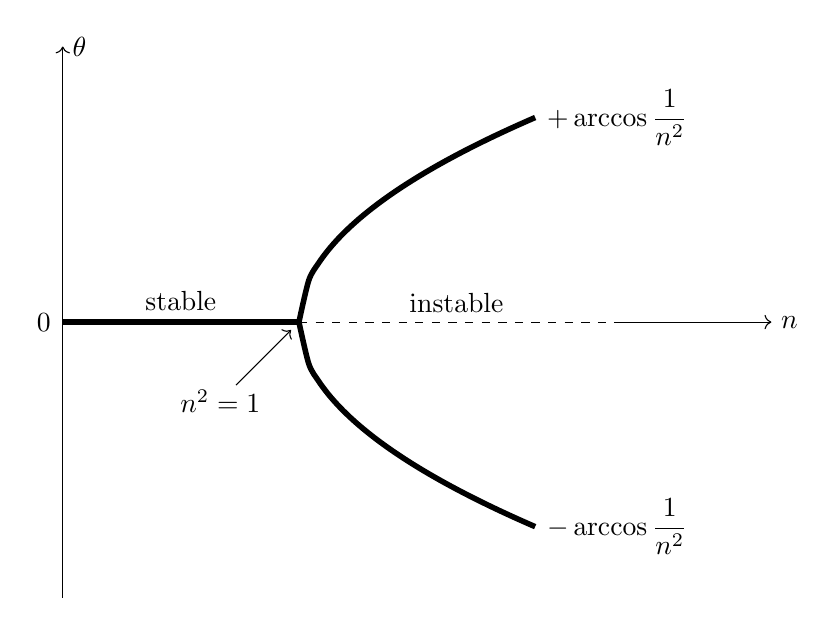
\begin{tikzpicture}
    \draw[->] (7,0) -- (9,0) node[right] {$ n $};
    \draw[->] (0,-3.5) -- (0,3.5) node[right] {$ \theta $};
    \draw[-, line width=2] node[left] {$ 0 $} (0,0) -- node[anchor=south]{stable} (3,0);
    \draw[-, dashed] (3,0) -- node[anchor=south]{instable} (7,0);

    \draw[color=black, smooth, line width=2, domain=3:6]   plot (\x,{ - 1.5 * sqrt(\x - 3) }) node[right]{$\displaystyle - \arccos \frac{1}{n^2} $};
    \draw[color=black, smooth, line width=2, domain=3:6]   plot (\x,{ + 1.5 * sqrt(\x - 3) }) node[right]{$\displaystyle + \arccos \frac{1}{n^2} $};
    
    \node [xshift = 2cm, yshift = -1cm] {$ n^2 = 1 $};
    \draw[->] (2.2,-0.8) -- (2.9,-0.1);

\end{tikzpicture} \end{center}





%% pendule rotatif autour d'un axe horizontal
\item Dans le cas où la courbe de guidage tourne autour d'un axe horizontal, la force de gravité n'est pas constante.


\NoIndent{
\begin{center}
\begin{tabular}{ccc}
%% Premier dessin
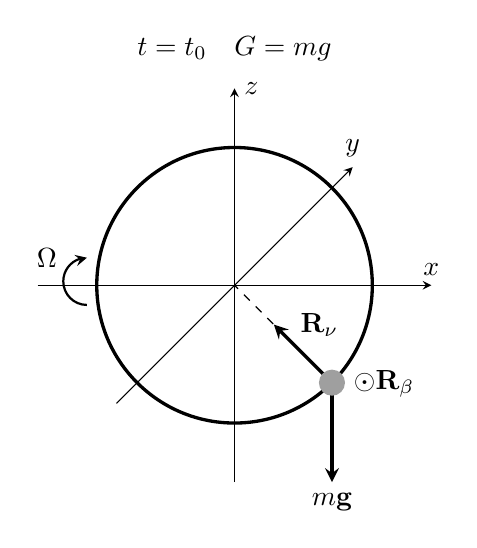
\begin{tikzpicture}[x=0.5cm,y=0.5cm,z=0.3cm,>=stealth]
\node [yshift=3cm] {$ t = t_0 \quad G = m g $};
% The axes
\draw[->] (xyz cs:x=-5) -- (xyz cs:x=5) node[above] {$x$};
\draw[->] (xyz cs:y=-5) -- (xyz cs:y=5) node[right] {$z$};
\draw[->] (xyz cs:z=-5) -- (xyz cs:z=5) node[above] {$y$};
% Circle
[x={(5cm,0cm)}, y={(-3cm,-3cm)}, z={(0cm,5cm)}, scale=0.2]
\tikzset{yxplane/.style={canvas is yx plane at z=#1}}
\begin{scope}[yxplane=0, very thick]
\draw (0,0) circle[radius=3.5cm];
\end{scope}
\draw [->, thick] (-3.75,-0.5) arc (-90:-270:.3cm) node[left, draw=none, xshift=-0.25cm, yshift=0cm]{$ \Omega $};
\draw [->, very thick] (2.4745,-2.4745) -- (2.4745,-5) node[below]{$ m \textbf{g} $};
\draw [-, dashed] (2.4745,-2.4745) -- (0,0);
\draw [->, very thick] (2.4745,-2.4745) -- (1,-1) node[right, xshift=0.2cm]{$ \textbf{R}_\nu $};
\node [draw=none] at (3.8,-2.5) {$ \odot \textbf{R}_\beta $};
\node [circle, xshift = 1.23725cm, yshift = -1.23725cm, fill=gray!75] {};
\end{tikzpicture}
&
%% Deuxième dessin
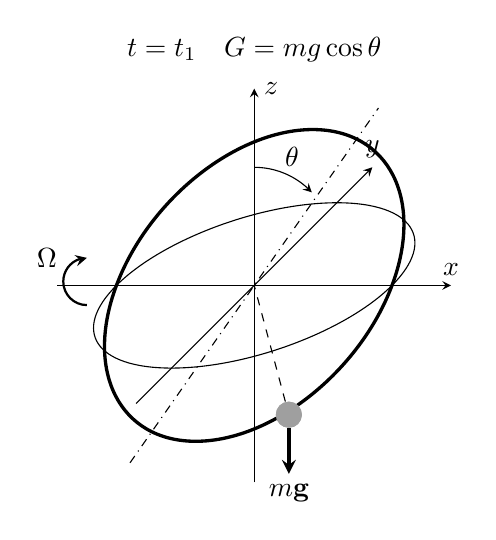
\begin{tikzpicture}[x=0.5cm,y=0.5cm,z=0.3cm,>=stealth]
\node [yshift=3cm] {$ t = t_1 \quad G = m g \cos \theta $};
% The axes
\draw[->] (xyz cs:x=-5) -- (xyz cs:x=5) node[above] {$x$};
\draw[->] (xyz cs:y=-5) -- (xyz cs:y=5) node[right] {$z$};
\draw[->] (xyz cs:z=-5) -- (xyz cs:z=5) node[above] {$y$};
% Circle
[x={(10cm,10cm)}, y={(-3cm,-3cm)}, z={(10cm,10cm)}, scale=0.2]
\tikzset{zxplane/.style={canvas is zx plane at y=#1}}
\begin{scope}[zxplane=0]
\draw (0,0) circle[radius=3.5cm] ;
\end{scope}
\draw [->, thick] (-4.25,-0.5) arc (-90:-270:.3cm) node[left, draw=none, xshift=-0.25cm, yshift=0cm]{$ \Omega $};
    \draw[very thick] (0,0,0) [y={(0,0.707,0.707)}] circle [radius=3.5];
\node (boule) at ($ (0,0) + (-75:3.4) $) [circle, xshift = 0cm, yshift = 0cm, fill=gray!75] {};
\draw [-, dashdotted] ($ (0,0) + (-125:5.5) $) -- ($ (0,0) + (55:5.5) $);
\draw [->, very thick] (boule) -- ($ (boule) - (0,1.5) $) node[below]{$ m \textbf{g} $};
\draw [-, dashed] (boule) -- (0,0);
\node () at ($ (0,0) + (-75:3.4) $) [circle, xshift = 0cm, yshift = 0cm, fill=gray!75] {};
\draw [->] (0,3) arc (90:43:1cm) node[above, draw=none, xshift=-0.25cm, yshift=0.2cm]{$ \theta $};
\end{tikzpicture}
&
%% Troisième dessin
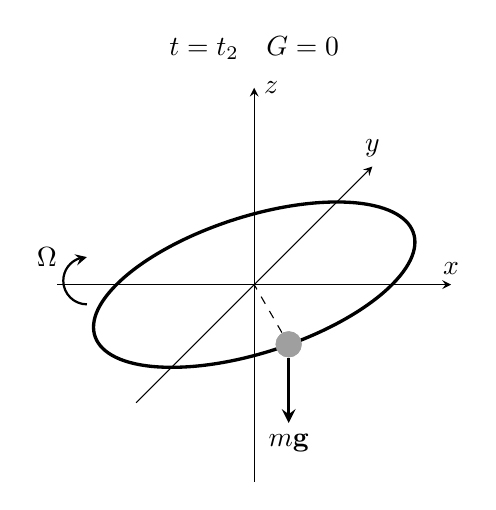
\begin{tikzpicture}[x=0.5cm,y=0.5cm,z=0.3cm,>=stealth]
\node [yshift=3cm] {$ t = t_2 \quad G = 0 $};
% The axes
\draw[->] (xyz cs:x=-5) -- (xyz cs:x=5) node[above] {$x$};
\draw[->] (xyz cs:y=-5) -- (xyz cs:y=5) node[right] {$z$};
\draw[->] (xyz cs:z=-5) -- (xyz cs:z=5) node[above] {$y$};
% Circle
[x={(5cm,0cm)}, y={(-3cm,-3cm)}, z={(0cm,5cm)}, scale=0.2]
\tikzset{zxplane/.style={canvas is zx plane at y=#1}}
\begin{scope}[zxplane=0, very thick]
\draw (0,0) circle[radius=3.5cm] ;
\end{scope}
\draw [->, thick] (-4.25,-0.5) arc (-90:-270:.3cm) node[left, draw=none, xshift=-0.25cm, yshift=0cm]{$ \Omega $};
\node (boule) at ($ (0,0) + (-60:1.75) $) [circle, xshift = 0cm, yshift = 0cm, fill=gray!75] {};
\draw [->, very thick] (boule) -- ($ (boule) - (0,2) $) node[below]{$ m \textbf{g} $};
\draw [-, dashed] (boule) -- (0,0);
\node () at ($ (0,0) + (-60:1.75) $) [circle, xshift = 0cm, yshift = 0cm, fill=gray!75] {};
\end{tikzpicture}
\end{tabular}
\end{center}}





\end{itemize}





















\section{Applications : Forces centrales}










\begin{itemize}





%% Forces centrales
\item Une force centrale est une force qui passe toujours par le même point, celui-ci est appelé centre de force. \\
Par exemple, la force d'attraction universelle est donnée par : $\displaystyle \textbf{F} = - \frac{G \; M m}{r^2} \textbf{e}_{r} $, et la force électrostatique s'écrit : $\displaystyle \textbf{F} = - \frac{1}{4 \pi \epsilon_0} \frac{q_1 q_1}{r^2} \textbf{e}_r $. La force centrale (en $ r^{-2} $) se note de manière générique ($ \mu > 0 $) : 
\[ \textbf{F} = - m \; \mu \; r^{-2} \; \textbf{e}_r \]






%% Conservation du moment cinétique des forces centrales
\item Le moment cinétique dû aux forces centrales est conservé puisque sa dérivée est nulle : $\displaystyle \textbf{s} \wedge \textbf{F} = m \textbf{s} \wedge \ddot{\textbf{s}} = \frac{d}{d t} \big[ m \textbf{s} \wedge \dot{\textbf{s}} \big] = 0 $ car $\displaystyle \frac{d}{d t} (\textbf{s} \wedge \dot{\textbf{s}}) = \underbrace{\dot{\textbf{s}} \wedge \dot{\textbf{s}}}_{0} + \textbf{s} \wedge \ddot{\textbf{s}} $. Le moment cinétique étant : $\displaystyle m \; \textbf{s} \wedge \dot{\textbf{s}} = \textbf{H}_0 $. 
\[ \textbf{s} \wedge \dot{\textbf{s}} = \textbf{h} \]
Ceci implique que le mouvement est plan ($ \textbf{s} \cdot \textbf{h} = 0 $ et $ \dot{\textbf{s}} \cdot \textbf{h} = 0 $).





%% Conservation de l'énergie
\item Il y a bien sûr conservation de l'énergie : $\displaystyle \frac{1}{2} m \| \dot{\textbf{s}} \|^2 + V = E $.





%% Constante h
\item On sait que : $ \textbf{s} = r \; \textbf{e}_r $ et $ \dot{\textbf{s}} = \dot{r} \; \textbf{e}_r + r \theta \; \textbf{e}_\theta $. D'où, $ \textbf{h} = \textbf{s} \wedge \dot{\textbf{s}} = r^2 \dot{\theta} \; \textbf{e}_z $
\[ \implies r^2 \dot{\theta} = h \]





%% Énergie
\item L'énergie du système vaut ($ \textbf{F} = - \nabla V $) : 
\begin{align*}
E &= T_O + V = \Big( \frac{1}{2} m \| \dot{\textbf{s}} \|^2 \Big) + \Big( - \mu m r^{-1} \Big) \\
&= \frac{1}{2} m \Big( \dot{r}^2 + \dot{r}^2 \dot{\theta}^2 \Big) - m \frac{\mu}{r} \\
&= \frac{1}{2} m \dot{r}^2 + \underbrace{m \frac{h^2}{2 \dot{r}^2} - m \frac{\mu}{r}}_{\mathpzc{V(r)}}
\end{align*}
On va comme dans la section précédente discuter du diagramme de potentiel de : 
\[ \tilde{\mathpzc{V}} = \frac{1}{2} \frac{h^2}{r^2} - \frac{\mu}{r} \]

\begin{center}
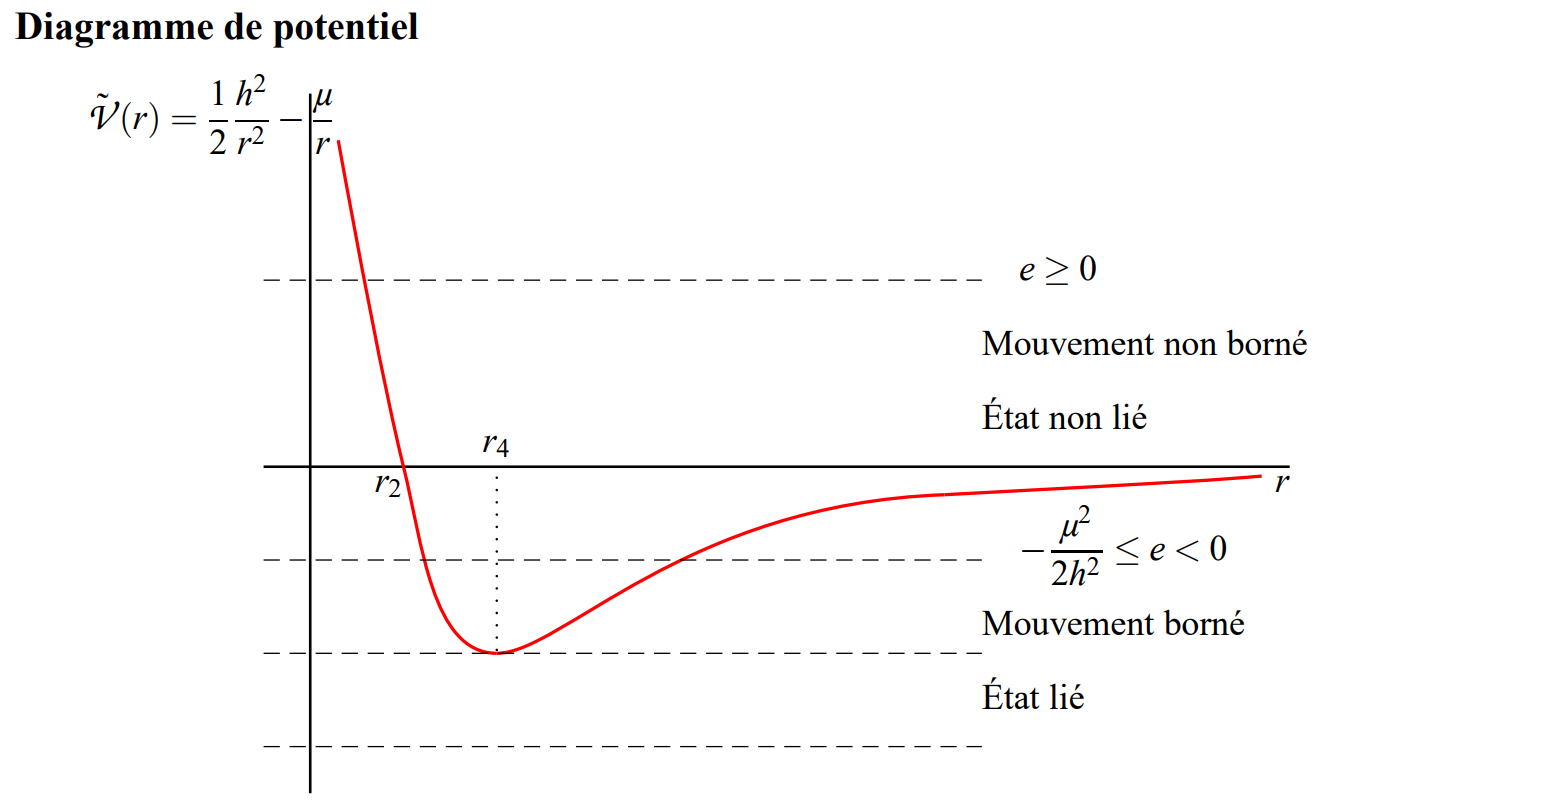
\includegraphics[width=0.9\textwidth]{images/forcecentrale.PNG}
\end{center}






%% Trajectoire
\item On cherche maintenant à déterminer exactement la trajectoire du système. Pour cela, on pose $ r = u^{-1} $ et $\displaystyle \frac{d r}{d u} = u^{-2} $.

\begin{center}
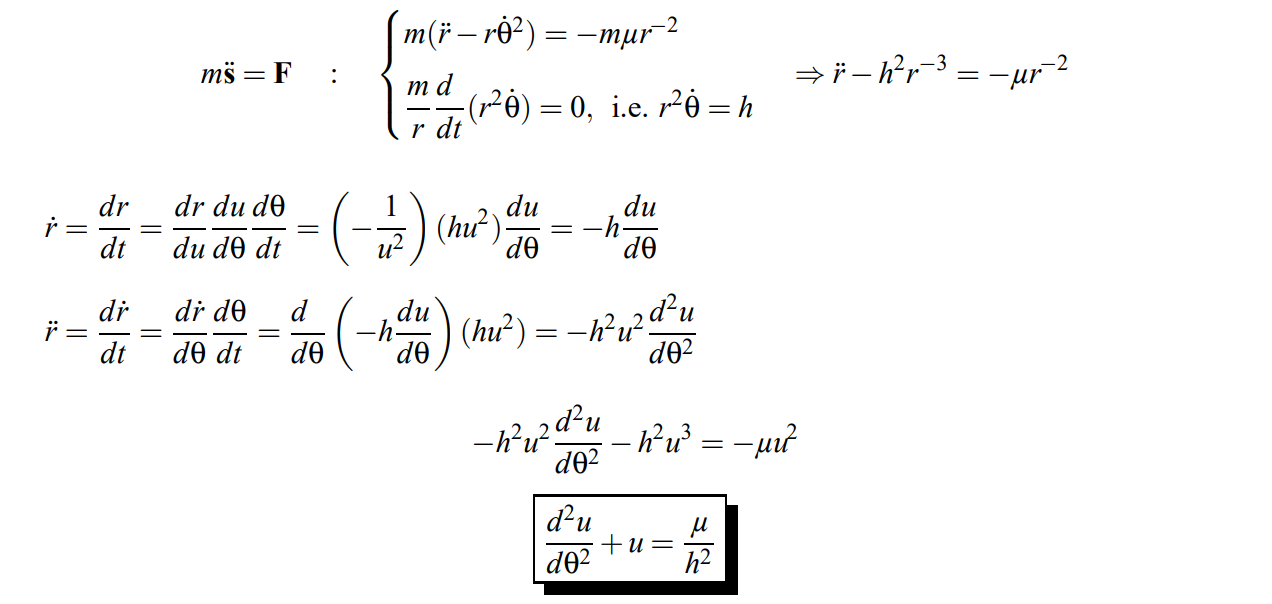
\includegraphics[width=0.8\textwidth]{images/trajectoire.PNG}
\end{center}

On tombe sur une équation différentielle facile à résoudre, sa solution est : 
\[ u(\theta) = A \cos \theta + B \sin \theta + \frac{1}{p} = \frac{1}{r(\theta)} \qquad \text{ où } p = \frac{h^2}{\mu} \]





%% Trajectoire conique
\item Fixons $ \theta = 0 $ lorsque $\displaystyle r = r_{min} = \frac{p}{1 + \epsilon} $ et posons $\displaystyle \epsilon = \sqrt{1 + \frac{2 e h^2}{\mu^2}} $. On a donc : 
\[ r(\theta) = \frac{p}{1 + \epsilon \cos \theta} \qquad \epsilon = \sqrt{1 + \frac{2 e h^2}{\mu^2}} \]
\begin{center}
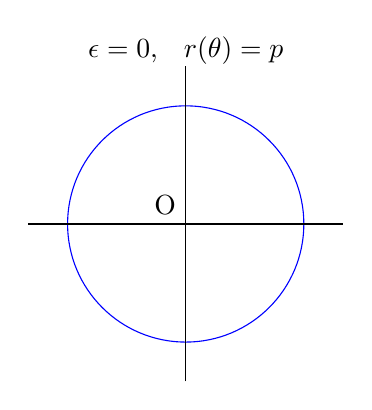
\begin{tikzpicture}
\draw [blue] circle [radius=1.5cm] (0,0);
\draw [-] (-2,0) -- (2,0);
\draw [-] (0,-2) -- node[anchor=south east]{O} (0,2);
\node [rectangle, draw=none, yshift=2.2cm] (0,0) {$ \epsilon = 0 $, \; $ r(\theta) = p $};
\end{tikzpicture}
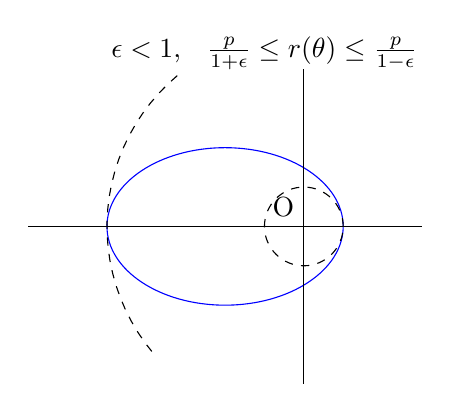
\begin{tikzpicture}
\draw (-1,0) [blue] ellipse (1.5cm and 1cm);
\draw [black, dashed] circle [radius=0.5cm] (0,0);
\draw [black, dashed, domain=130:220] plot ({2.5*cos(\x)}, {2.5*sin(\x)});
\draw [-] (-3.5,0) -- (1.5,0);
\draw [-] (0,-2) -- node[anchor=south east]{O} (0,2);
\node [rectangle, draw=none, yshift=2.2cm, xshift=-0.5cm] (0,0) {$ \epsilon < 1 $, \; $ \frac{p}{1 + \epsilon} \leq r(\theta) \leq \frac{p}{1 - \epsilon} $};
\end{tikzpicture}
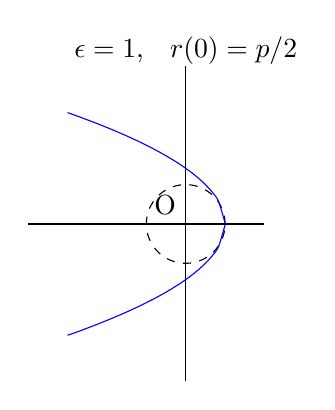
\begin{tikzpicture}
\draw [black, dashed] circle [radius=.5cm] (0,0);
\draw [-] (-2,0) -- (1,0);
\draw [-] (0,-2) -- node[anchor=south east]{O} (0,2);
\node [rectangle, draw=none, yshift=2.2cm] (0,0) {$ \epsilon = 1 $, \; $ r(0) = p/2 $};
\draw[color=blue, smooth, domain=-2:0, xshift=0.5cm] plot (\x,{ sqrt(- \x) });
\draw[color=blue, smooth, domain=-2:0, xshift=0.5cm] plot (\x,{ - sqrt(- \x) });
\end{tikzpicture}
\end{center}

\begin{center}
$ \epsilon > 1, \; r(0) = \frac{p}{1 + \epsilon} $ \\
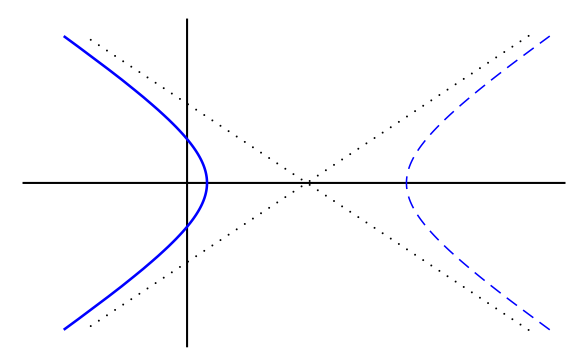
\includegraphics[width=0.4\textwidth]{images/hyperbole.PNG}
\end{center}






%% Lois de Kepler sur le mouvement des planètes
\item Lois de Kepler sur le mouvement des planètes : 
\begin{enumerate}
\item Les trajectoires des planètes sont des ellipses dont le Soleil est un des foyers.
\item Le rayon vecteur joignant le soleil à une planète balaie des aires égales en des temps égaux au cours de son mouvement autour du soleil.
\item Le carré des périodes des mouvements planétaires sont proportionnels aux cubes des grands axes des trajectoires.
\end{enumerate}





%% 2ème Loi de Kepler
\item Démonstration de la $ 2^{\text{ème}} $ loi de Kepler : 

\begin{center}
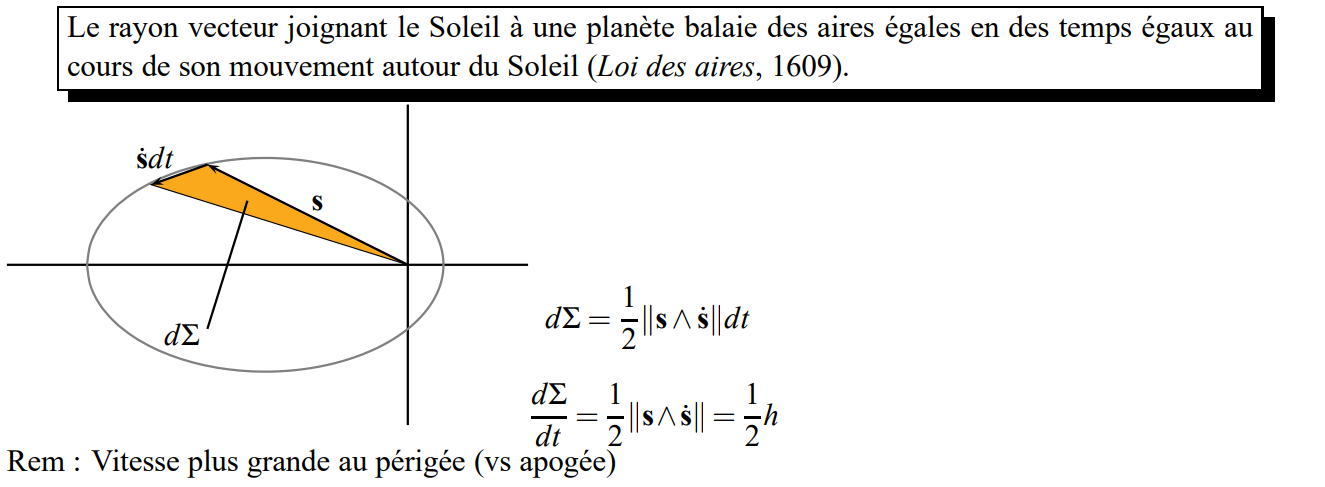
\includegraphics[width=0.9\textwidth]{images/AireKepler.PNG}
\end{center}






%% 3ème Loi de Kepler
\item Démonstration de la $ 3^{\text{ème}} $ loi de Kepler : 

\begin{center}
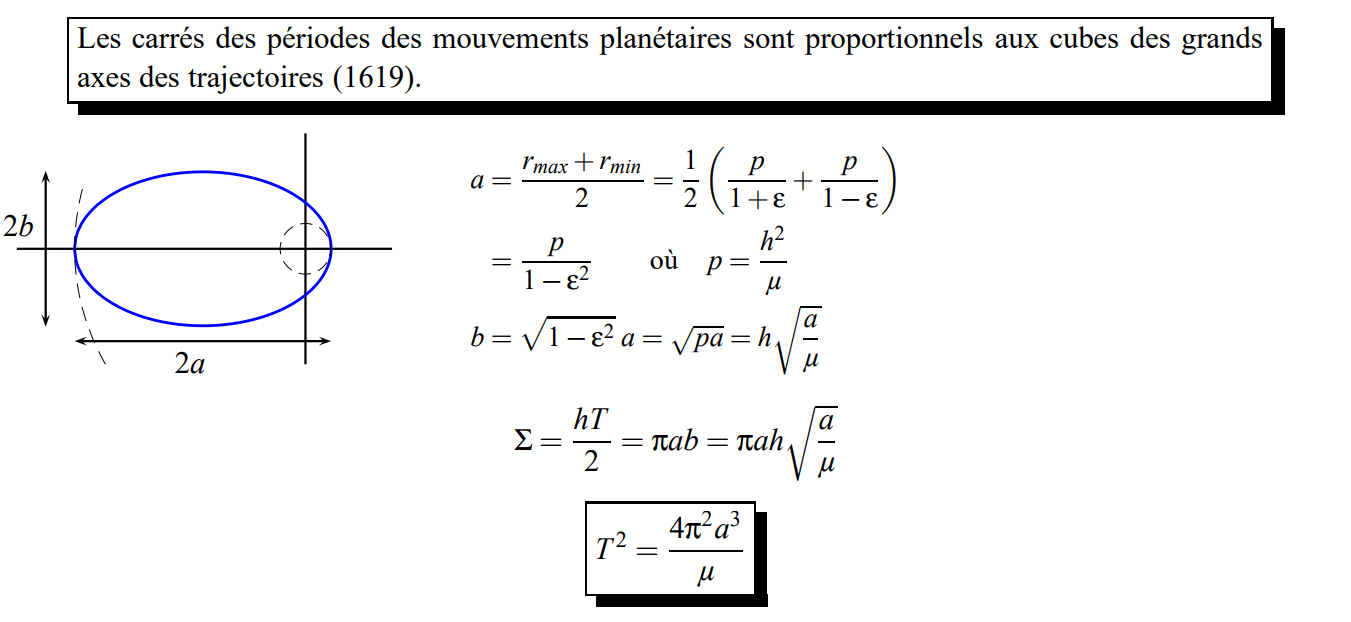
\includegraphics[width=0.9\textwidth]{images/RevolutionKepler.PNG}
\end{center}





\end{itemize}




















\section{Applications : Caractéristiques du solide}










\begin{itemize}





%% Centre d'inertie
\item Le point \emph{C} (centre d'inertie) est tel que : 
\[ \begin{aligned} m \; \textbf{c} &= \begin{cases} \textbf{Q}_O \\ \text{moment statique} \end{cases} \\ &= \int_{\text{solide}} \textbf{s} \; d m \end{aligned} \]
où le vecteur \textbf{s} balaie l'ensemble du solide.

\begin{center} 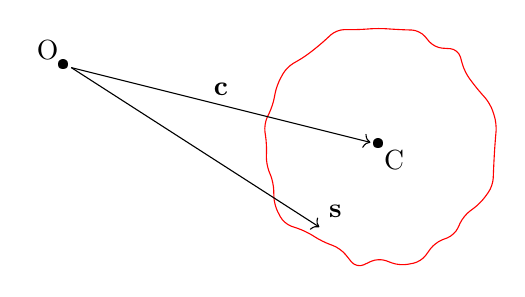
\begin{tikzpicture}
\coordinate (O) at (0,0);
\coordinate (c) at (4,-1);
\draw [red,rounded corners=1mm] (c) \irregularcircle{1.5cm}{1mm};

\node [] at (O) {\textbullet}; \node [yshift=0.2cm, xshift=-0.2cm] at (O) {O};
\node [] at (c) {\textbullet}; \node [yshift=-0.2cm, xshift=0.2cm] at (c) {C};

\draw [->] ($ (O) + (0.1,-0.025) $) -- node[midway, yshift = 0.2cm]{\textbf{c}} ($ (c) - (0.1,-0.025) $);
\draw [->] ($ (O) + (0.1,-0.025) $) -- ($ (c) - (0.75,1.05) $) node[right, yshift = 0.2cm]{\textbf{s}};
\end{tikzpicture} \end{center}

\begin{itemize}
\item[*] Le point C se situe sur un élément de symétrie matérielle su solide.
\item[*] Théorèmes de Guldin : 
    \begin{enumerate}
    \item Premier théorème : 

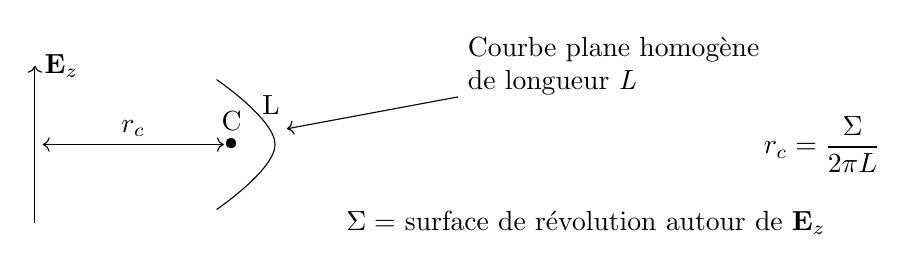
\begin{tikzpicture}
\coordinate (c) at (2.5,0);
\draw [->] (0,-1) -- (0,1) node[right]{$ \textbf{E}_z $};
\node [] at (c) {\textbullet}; \node [yshift=0.3cm] at (c) {C};
\draw [<->] (0.1,0) -- ($ (c) - (0.1,0) $) node[midway, yshift=0.2cm]{$ r_c $};

\draw  plot[smooth, tension=.7, scale=0.55] coordinates {($ (c) - (0.35,1.5) $) ($ (c) + (1,0) $) ($ (c) + (-0.35,1.5) $)};

\node (L) [] at ($ (c) + (0.5,0.5) $) {L};
\node (texte1) [text width=4cm] at ($ (c) + (5,1) $) {Courbe plane homogène de longueur \emph{L}};

\draw [->] (texte1) -- ($ (L) - (-0.2,0.3cm) $);
\node [] at (10,0) {$\displaystyle r_c = \frac{\Sigma}{2 \pi L} $};
\node [] at (7,-1) {$ \Sigma = $ surface de révolution autour de $ \textbf{E}_z $};
\end{tikzpicture}

    \item Second théorème : 

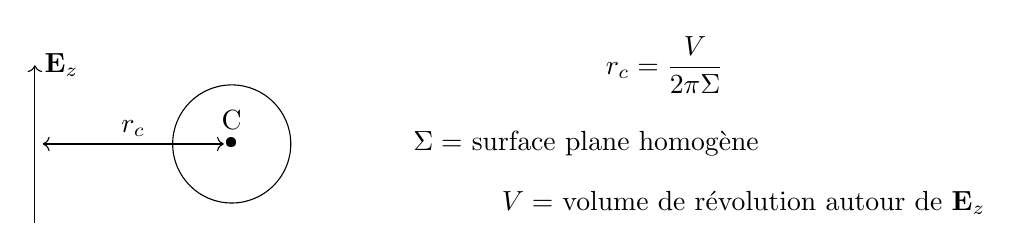
\begin{tikzpicture}
\coordinate (c) at (2.5,0);
\draw [->] (0,-1) -- (0,1) node[right]{$ \textbf{E}_z $};
\node [] at (c) {\textbullet}; \node [yshift=0.3cm] at (c) {C};
\draw [<->] (0.1,0) -- ($ (c) - (0.1,0) $) node[midway, yshift=0.2cm]{$ r_c $};

\draw [black, xshift=2.5cm] circle [radius=0.75cm];

\node [] at (8,1) {$\displaystyle r_c = \frac{V}{2 \pi \Sigma} $};
\node [] at (7,0) {$ \Sigma = $ surface plane homogène};
\node [] at (9,-0.75) {$ V = $ volume de révolution autour de $ \textbf{E}_z $};
\end{tikzpicture}
    \end{enumerate}
\item[*] Principe de superposition : 
    \begin{enumerate}
    \item[(a)] Sans encoche : \\
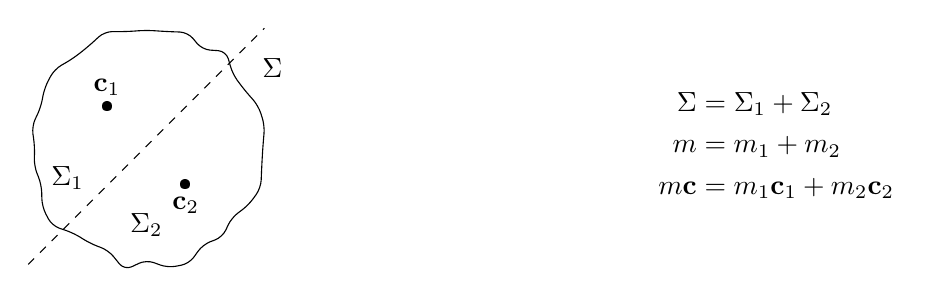
\begin{tikzpicture}
\draw [rounded corners=1mm] \irregularcircle{1.5cm}{1mm};
\draw [-, dashed] (-1.5,-1.5) -- (1.5,1.5);

\node [yshift=-1cm] {$ \Sigma_2 $};
\node [yshift=-0.4cm, xshift=-1cm] {$ \Sigma_1 $};
\node [yshift=1.cm, xshift=1.6cm] {$ \Sigma $};

\node (c1) [xshift=-0.5cm, yshift=0.5cm] {\textbullet}; \node [yshift=0.25cm] at (c1) {$ \textbf{c}_1 $};
\node (c2) [xshift=0.5cm, yshift=-0.5cm] {\textbullet}; \node [yshift=-0.25cm] at (c2) {$ \textbf{c}_2 $};

\node [] at (8,0) {$ \begin{aligned} \Sigma &= \Sigma_1 + \Sigma_2 \\ m &= m_1 + m_2 \\ m \textbf{c} &= m_1 \textbf{c}_1 + m_2 \textbf{c}_2 \end{aligned} $};
\end{tikzpicture}

    \item[(b)] Avec encoche : \\
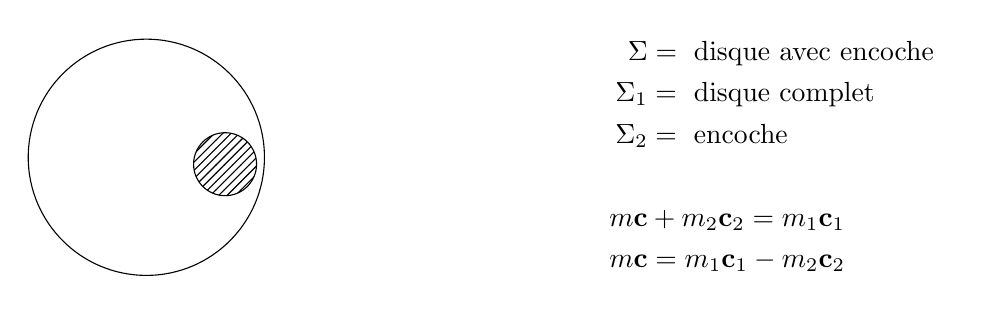
\begin{tikzpicture}
\draw [black] circle [radius=1.5cm];
\draw [black, xshift=1cm, yshift=-2.5, fill=white, fill, pattern=north east lines] circle [radius=0.4cm];

\node [] at (8,0) {$ \begin{aligned} \Sigma &= \text{ disque avec encoche } \\ \Sigma_1 &= \text{ disque complet } \\ \Sigma_2 &= \text{ encoche } \\ & \\ m \textbf{c} &+ m_2 \textbf{c}_2 = m_1 \textbf{c}_1 \\ m \textbf{c} &= m_1 \textbf{c}_1 - m_2 \textbf{c}_2 \end{aligned} $};
\end{tikzpicture}
    \end{enumerate}
\end{itemize}





%% Calcul du tenseur d'inertie
\item Le tenseur d'inertie par rapport à un point \emph{B} est donné par : $\displaystyle \textbf{J}_B = \int_{\text{solide}} \big( \textbf{s}^2 \textbf{I} - \textbf{s} \textbf{s} \big) \; dm $, où \textbf{I} est le tenseur identité et \textbf{s} est le vecteur position par rapport à \emph{B}.
\[ J_B = \int \begin{pmatrix} y^2 + z^2 & - x y & - x z \\ - x y & x^2 + z^2 & - y z \\ - x z & - y z & x^2 + y^2 \end{pmatrix} \; d m \]
La matrice est symétrique, donc diagonalisable. Dés lors, il existe un repère dans lequel $ J_B $ est représenté par une matrice diagonale. \\
Les axes du repères sont les : 
\begin{itemize}
\item Vecteurs propres du solide.
\item Axes principaux du solide.
\item Axes de symétries du solides (s'ils existent).
\end{itemize}
On exprime $ \textbf{J}_B $ : 
\begin{itemize}
\item[*] Dans les axes principaux d'inertie (seulement trois intégrales à calculer).
\item[*] Dans les axes liés au solide ($ \textbf{J}_B $ constant).
\item[*] En 0, point fixe du solide. \\ En C, centre d'inertie du solide.
\end{itemize}

Soient $ C, \textbf{e}_1, \textbf{e}_2, \textbf{e}_3 $ les a.p.i. (= axes principaux d'inertie) liés au solide en \emph{C}. On a : $ \textbf{s} = x_1 \textbf{e}_1 + x_2 \textbf{e}_2 + x_3 \textbf{e}_3 $ et : $ J_C = \begin{pmatrix} J_1 & 0 & 0 \\ 0 & J_2 & 0 \\ 0 & 0 & J_3 \end{pmatrix} = \text{ diag } (J_1, J_2, J_3) $ dans la base des $ \textbf{e}_i $ (base des a.p.i.).


\begin{tikzpicture}[overlay,remember picture]
        \draw[thick,blue,fill=blue!20,rounded corners] 
            ($(pic cs:m1)+(-0.05,0.4)$) -- ($(pic cs:m2)+(0.05,0.4)$) -- 
            ($(pic cs:m6)+(0.05,-0.4)$) -- ($(pic cs:m5)+(-0.05,-0.4)$) -- cycle; 
        \draw[blue,thick,-latex] ($(pic cs:m5)+(0.1,-0.4)$) to [in=180,out=15] +(-15:1cm) 
            node[anchor=west,text=black] {Moments principaux d'inertie};
    \end{tikzpicture}
\begin{equation*} \begin{cases} \displaystyle
\tikzmark{m1}J_1\tikzmark{m2} = \int \Big( x_2^2 + x_3^2 \Big) \; d m \\ \displaystyle
\tikzmark{m3}J_2\tikzmark{m4} = \int \Big( x_1^2 + x_3^2 \Big) \; d m\\ \displaystyle
\tikzmark{m5}J_3\tikzmark{m6} = \int \Big( x_1^2 + x_2^2 \Big) \; d m
\end{cases} \end{equation*}

\[  \] %%   Sert à espacer les blocs d'équations correctement
\[ \textbf{J}_C = J_1 \textbf{e}_1 \textbf{e}_1 + J_2 \textbf{e}_2 \textbf{e}_2 + J_3 \textbf{e}_3 \textbf{e}_3 \]





%% Cas particuliers : moments d'inertie et axes principaux d'inertie
\item Cas particuliers : moments d'inertie et axes principaux d'inertie
\begin{enumerate}
\item[(a)] Système rectiligne : Il suffit de calculer un seul moment d'inertie par rapport à une droite perpendiculaire à la droite du solide.
\item[(b)] Système plan : (plan $ Oxy $, $ z = 0 $)
\[ J_x = \int y^2 \; d m \qquad ; \qquad J_y = \int x^2 \; d m \qquad ; \qquad J_z = \int \Big( x^2 + y^2 \Big) \; d m \]
Et donc : $\displaystyle J_x + J_y = J_z \qquad ; \qquad J_{y z} = J_{x z} = 0 $ et l'ellipsoïde d'inertie est donné par : 
\[ J_x x^2 + J_y y^2 + (J_x + J_y) z^2 - 2 J_{x y} x y = 1 \]
Son intersection avec le plan $ Oxy $ ($ z = 0 $) donne l'ellipse d'inertie d'équation : 
\[ J_x x^2 + J_y y^2 - 2 J_{x y} x y = 1 \]
\item[(c)] Le système possède un axe de symétrie : Prenons cet axe pour $ Oz $. On a : 
\[ J_{y z} = J_{x z} = 0 \]
Ceci implique que l'\emph{axe de symétrie} est un axe principal d'inertie. Et puisqu'il porte le centre d'inertie, il est l'un des \emph{axes centraux principaux d'inertie}.
\item[(d)] Le système possède un axe de symétrie\footnote{Un axe de symétrie est d'ordre \emph{n} si une rotation de $\displaystyle \frac{2 \pi}{n} $ autour de cet axe transforme le solide en lui-même.} d'ordre \emph{n} (avec $ n \neq 2 $) : L'ellipsoïde d'inertie est de révolution autour de cet axe.
\item[(e)] Le système possède un plan de symétrie : Toute droite perpendiculaire au plan de symétrie est principale d'inertie. Car $ J_{y z} = 0 $ et $ J_{x z} = 0 $.
\end{enumerate}





%% Quelques informations à propos du tenseur d'inertie
\item Quelques informations à propos du tenseur d'inertie : 
\begin{itemize}
    \item[*] Le théorème C donne la formule : $\displaystyle \textbf{J}_O = \textbf{J}_C + m \; \Big[ c \; \textbf{I} - \textbf{c} \textbf{c} \Big] $. \qquad \big( \danger Important ! \big)
    \item[*] Le moment d'inertie par rapport à une droite \emph{d} et de direction \textbf{e} passant par \emph{B} est donné par : $ J_B^d = \textbf{e} \cdot \textbf{J}_B \cdot \textbf{e} $ \qquad où \textbf{e} est unitaire.
    \item[*] Le théorème de transport est un théorème qui donne le moment d'inertie autour d'une droite $ d_1 $ passant par \emph{O} parallèle à $ d_2 $ passant par \emph{C} : $\displaystyle J_O^{d_1} = J_C^{d_2} + m l^2 $.

\end{itemize}






\end{itemize}




















\section{Applications : Mouvement du solide}










\begin{itemize}





%% Dynamique du solide : Théorème généraux
\item Dynamique du solide : Théorème généraux : \\
Un solide indéformable peut avoir jusqu'à six degrés de liberté (3 de translation et 3 de rotation), pour déterminer le mouvement d'un solide, on a donc affaire à 6 inconnues.
\[
\left.\begin{aligned}
\text{ Th. I } \quad & m \ddot{\textbf{c}} = \textbf{G} \quad & 3 \text{ équations } \\
\text{ Th. II } \quad & \dot{\textbf{H}}_O = \textbf{M}_O \quad & 3 \text{ équations } \\
\text{ Th. II}_C \quad & \dot{\textbf{H}}_C = \textbf{M}_C \quad & 3 \text{ équations } \\
\text{ Th. III } \quad & \dot{T}_O = \mathpzc{P}_O \quad & 1 \text{ équation } \\
\text{ Th. III}_C \quad & \dot{T}_C = \mathpzc{P}_C \quad & 1 \text{ équation }
\end{aligned}\right\rbrace \qquad \implies 11 \text{ inconnues }
\]
Il y a donc plusieurs approches possibles dans la résolution des problèmes. \\
Classiquement : 
\[ \text{ Th. I (mouvement de \emph{C}) \quad + \quad Th. II}_C \text{ (mouvement autour de \emph{C}) }  \]
\[ \longrightarrow \text{ 6 éq. pour 6 inconnues } \]





%% Méthodes de l'étude du mouvement d'un solide
\item Méthodes de l'étude du mouvement d'un solide : \\
\NoIndent{
\begin{tabular}{p{8cm}|p{8cm}}
\multicolumn{1}{c|}{Méthode 1}  & \multicolumn{1}{c}{Méthode 2} \\ \hline
\textcircled{+} Si on étudie seulement le mouvement     & \textcircled{+} Toujours possible \\
\textcircled{-} Seulement si il y a conservation de l'énergie   & \textcircled{-} Système à résoudre \\
\hdashline
\begin{enumerate}
\item[(a)] Il faut démontrer la conservation de l'énergie (ex : forces appliquées = conservatives \& forces de réaction ne développent pas de puissance)
\item[(b)] On utilise le \underline{Th. III en \emph{O}} = théorème de l'énergie cinétique en \emph{O} (axes absolus en \emph{O}) : 
\[ \dot{T}_O = \mathpzc{P}_O \]
avec $ T_O + V = E \; \longrightarrow \; $ 1 éq. pour \emph{O}
\item[(c)] On utilise le \underline{Th. I} = théorème de la quantité de mouvement (axes absolus en \emph{O}) : 
\[ \dot{\textbf{N}}_O = \textbf{G}^{\text{ext}} \]
projeté sur $ \textbf{E}_x $ \& $ \textbf{E}_y $ donne $ \textbf{R}_m $ et $ \textbf{R}_n $ en fonction de $ \theta $.
\end{enumerate} & \begin{enumerate}
\item[(a)] On utilise le \underline{Th. I} = théorème de la quantité de mouvement (axes absolus en \emph{O}) : 
\[ \dot{\textbf{N}}_O = \textbf{G}_{\text{ext}} \]
projeté sur $ \textbf{E}_x $ \& $ \textbf{E}_y $ donne $ \textbf{R}_m $ et $ \textbf{R}_n $ en fonction de $ \theta $.
\item[(b)] On utilise le \underline{Th. II} = théorème du moment cinétique (axes absolus en O) : 
\[ \dot{\textbf{H}}_O = \textbf{M}_O^{\text{ext}} \]
projeté sur $ \textbf{E}_z \longrightarrow $ 1 éq. si mouvement plan
\end{enumerate}
\end{tabular} }





%% Mouvement plan
\item Un solide est en mouvement plan lorsque 3 des ses points non alignés se déplacent à chaque instant dans un même plan. \\
On dit aussi que pour qu’un solide soit en mouvement plan, il faut que la résultante des forces soit dans le plan du mouvement et que le moment résultant par rapport au centre d’inertie soit perpendiculaire à celui-ci





%% Pendule plan
\item Pendule plan : 
\begin{center} 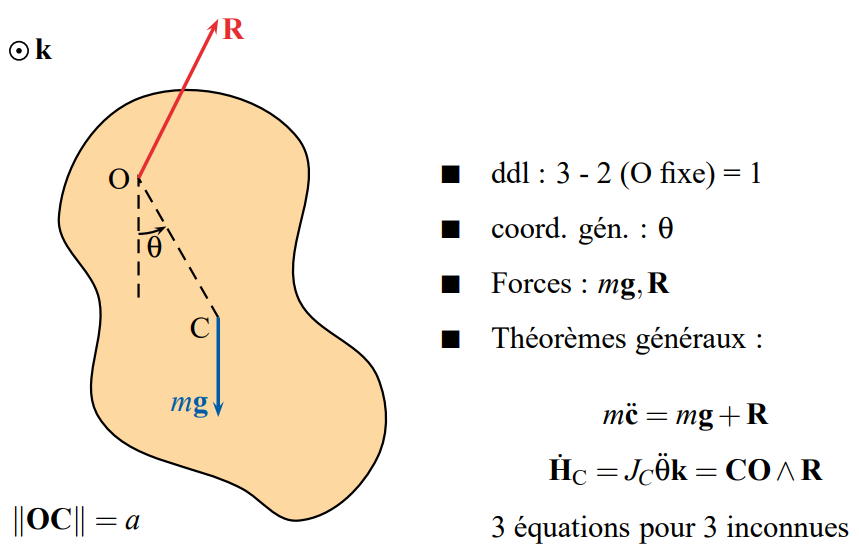
\includegraphics[width=0.5\textwidth]{images/PendulePlan.PNG} \end{center}
Centre d'oscillation : 
\begin{center} 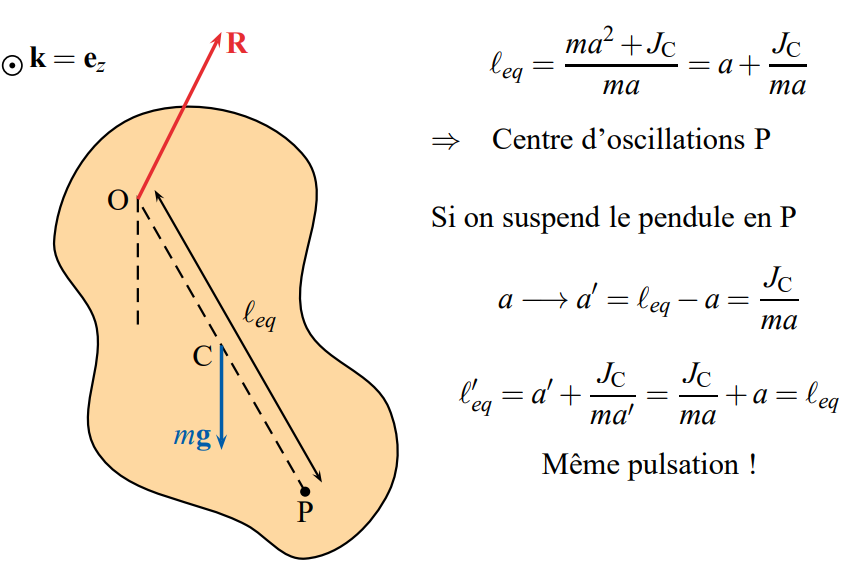
\includegraphics[width=0.5\textwidth]{images/COscillation.PNG} \end{center}
Centre de percussion : 
\begin{center} 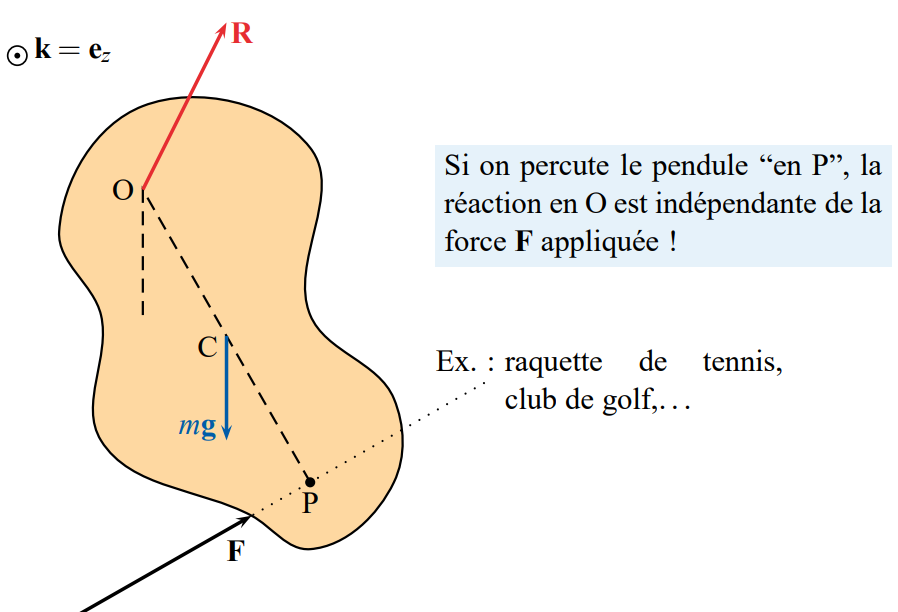
\includegraphics[width=0.5\textwidth]{images/CPercussion.PNG} \end{center}





%% -> Change l'espacement entre les lignes du tableau
\renewcommand{\arraystretch}{2}





%% Mouvements des solides dans l'espace
\item Mouvements des solides dans l'espace $ \longrightarrow $ voir "Lesson 9". \danger Grand risque d'avoir ça à l'examen \danger \\
Résumé (méthodes de résolution : mouvement des solides dans l'espace) : 
\begin{center} \begin{tabular}{c|c|c}
& \emph{Roulement sans glissement}    & \emph{Roulement avec glissement} \\ \hline
\emph{Équations}    & Théorèmes généraux +  & Théorèmes généraux + \\
& $\displaystyle \textbf{v}_K = \textbf{0} $ & $\displaystyle \textbf{T} = - \mu | N | \frac{\textbf{v}_K}{\| \textbf{v}_K \|} $ \\[0.3cm] \hline
\emph{Hypothèses}   & $ \| \textbf{T} \| \leq \mu N \; ? $ & $ \| \textbf{v}_K \| \neq 0 \; ? $ \\
& Oui : OK & Oui : OK \\[-0.4cm]
& Non : Phase avec glissement & Non : Phase sans glissement
\end{tabular} \end{center}





\end{itemize}













\end{document}}